\chapter{Hydrodynamic and sedimentary analysis}
\label{chap:hydroanalysis}
\section{Effect of tides and waves on the water level}

\subsection{Tides, waves and currents}
In addition to the study on the effects of sand mining on the river bed, it is as important to look at the effects of water on the river banks. Relevant to this project, the two situations that contribute to this problem are the elevation of the water level due to the high astronomical tide, and the elevation of the water level due to the ship waves.

\subsubsection{Astronomical tides}

Tide is the rise and fall of the water level, in particular the sea level, due to the gravitational force of the moon \autocite{nationaloceanicandatmosphericadministrationTidesCurrents}. As said, the tidal influence is the strongest in the ocean, pulling away the sea from one side of the globe to the other depending on the position of the moon. 
This gravitational force can also apply to rivers, as long as they are part of, or near a substantial quantity of water mass. Since the region of interest is situated in the Lower Paraná Delta, it is expected to be tidally influenced by the Río de la Plata. Therefore, tidal effects are of significance for the data analysis. This will be treated in section \ref{sec:tidal forcing}.

\subsubsection{Waves}

The gravitational force not only yields a change in water level, but is also responsible for tidal waves. These are induced by the gravitational pull, in the direction of the moving current. 
In addition to that, there are also wind waves. These are produced by a striking distance called the fetch, where the wind blows on the surface of the water, gathering energy which translates into a wave. In order to find the significant wave height of this situation, one takes a sample of wave heights from buoys and takes the average of the highest third waves \autocite{arrigaLecture2CIEM40002025}.

Given that the river is not straight, the fetch or striking distance is usually quite short, as seen in Figure \ref{Figure 1.1}. This means that the impact of the wind waves can theoretically only be quite small. Therefore, this impact will not be taken into consideration.

The last part of the waves that will be treated in this subsection are the ship waves. These are created when a ship passes by and pushes away the water to make way for the boat to go forward. This situation initiates three types of waves: primary, secondary, and propeller wash waves. These can be seen in Figure \ref{Fig:Ship Waves Effect on Water and Bank} \autocite{antoniniLecture12Ships2025}. The impact of the secondary wave is the most promiscuous, as one can tell from the frequency plot underneath the sketch in Figure \ref{fig:Prop Wash Wave}. 

\begin{figure}[H]
    \centering
    % First subfigure
    \begin{subfigure}{0.48\linewidth}
        \centering
        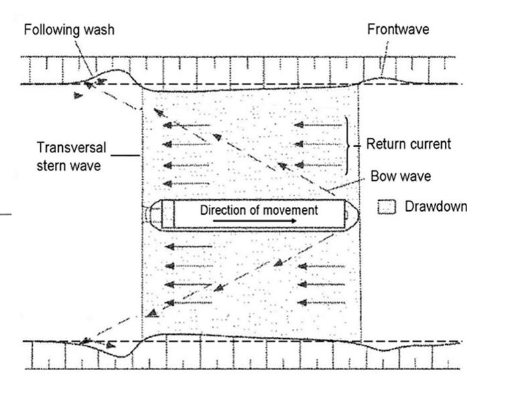
\includegraphics[width=\linewidth]{figures/ch2/shipwaves.png}
        \caption{Ship Waves}
        \label{fig:Ship Waves}
    \end{subfigure}
    \hfill
    % Second subfigure
    \begin{subfigure}{0.48\linewidth}
        \centering
        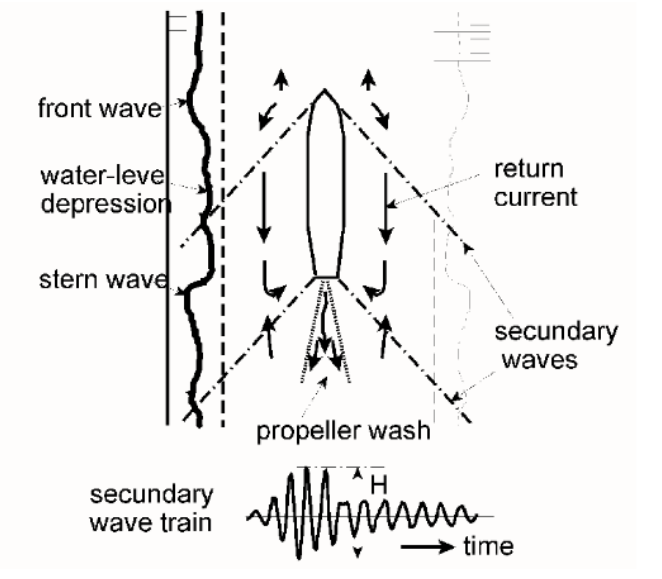
\includegraphics[width=\linewidth]{figures/ch2/shipsecond.png}
        \caption{Propeller Wash Wave}
        \label{fig:Prop Wash Wave}
    \end{subfigure}
    \caption{Ship Waves Effect on Water and Bank}
    \label{Fig:Ship Waves Effect on Water and Bank}
\end{figure}



\subsubsection{Currents}

Due to changes in water level as well as supplementary waves, a change in current applies. Using the standard values of the Netherlands and the given facts about the size of the ships circulating and the currents in the Rio Paraná Guazú, one could assume the wave height and current amplitudes for this case. This can be reflected once the field measurements are known, as described in Section \ref{sec:field study}.
Table \ref{tab:standard_values} gives the standard design values for wave heights and currents. Understandably, the relevant row for this project is the 'Rivers' category. Hinting to the fact that big ships are usually present in the channel, one might take values towards the upper boundary of the table.

\begin{table}[H]
    \centering
    \caption{Standard values for wave heights and currents in the Netherlands (Data from CUR 197 ``Breuksteen in de praktijk'').}
    \label{tab:standard_values}
    \begin{tabular}{lcccc}
        \toprule
        Location & \multicolumn{2}{c}{Wave heights (m)} & \multicolumn{2}{c}{Currents (m/s)} \\
        \cmidrule(lr){2-3} \cmidrule(l){4-5}
        & Wind waves & Ship waves & Natural current & Return current \\
        \midrule
        Lakes          & 0.25 -- 1.00  & 0.10 -- 0.50  & 0.1 -- 0.5  & 0.1 -- 0.25 \\
        Canals         & 0.10 -- 0.25  & 0.25 -- 0.75  & 0.5 -- 1.0  & 0.5 -- 1.0  \\
        Rivers         & 0.25 -- 1.00  & 0.25 -- 0.75  & 1.0 -- 2.0  & 0.5 -- 1.0  \\
        Small waters   & 0.10 -- 0.20  & n.a.          & 0.2 -- 1.0  & n.a.       \\
        \bottomrule
    \end{tabular}
\end{table}


\subsection{Loads and Impacts due to Ships}
Following the information about tides, waves and currents one might ask how the ship induced waves may exert a force on the river bed. This can be done with the help of wave theory. The first relevant parameters to take into account are the ship waves in rivers. These are assumed to be between 0.25 and 0.75 meters tall according to Table \ref{tab:standard_values}. Based on observations during the field trip, the value of 0.25 meter wave height is chosen as the cargo ships do not travel with a speed significant enough to reach a height of 0.75 m at the riverbed 100 meters away.
There are two types of currents comning from the ship, the natural and return current. Since the natural current is the relevant one in this case due to its magnitude of 1.5 [m/s] compared to 0.5 [m/s] \ref{tab:standard_values} will serve as a reference for further calculations \autocite{hasanShipinducedWaveForces2025}.
This gives the following parameters:

\begin{table}[H]
    \centering
    \caption{Design Parameters for Wave Impact Calculation}
    \label{tab:Parameters for Wave Impact Calculation}
    \begin{tabular}{lcc}
        \toprule
        Location & Ship wave height: H (m) & Natural current: u (m/s) \\
        \midrule
        Rivers & 0.25 & 1.5 \\
        \bottomrule
    \end{tabular}
\end{table}

\subsubsection{Wave Load}
Next, one can calculate the force of the wave, assuming that the wave signal given by the boat is uniform. In the calculation one assumes from the video filmed in the field trip that the wave spectrum coming from the ship includes about 10 repetitions, and that the boat is located 100 meters from the shore. This leaves us with the wave theory of \autocite{arrigaLecture2CIEM40002025} which states that there are two types of waves you can get energy from:

\begin{itemize}
    \item Periodic waves 
    \item Random waves 
\end{itemize}

Wave energy is a specific energy and it is calculated per unit of horizontal area [J/m$^2$]. The equation to calculate wave power for periodic and random waves is given as follows:

\begin{equation}
\label{eq:periodic wave energy}
    {E_{pw} = \left(\frac{1}{8}\right) \cdot \rho \cdot g \cdot H_{m0}^2}
\end{equation}

\begin{equation}
\label{eq:random wave energy}
    {E_{rw} = \left(\frac{1}{16}\right) \cdot \rho \cdot g \cdot H_{m0}^2}
\end{equation}

\noindent where:
\begin{itemize}
    \item $\rho$ is the density of fresh water: 1000 [kg/m\textsuperscript{3}];
    \item \(H_{m0}^2\) is the wave height: 0.50 [m\textsuperscript{2}];
    \item \(g\) is the gravitational constant: 9.81 [m/s\textsuperscript{2}]
\end{itemize}

On a small interval of time, the ship waves can be assumed to be periodic. Therefore, Equation \ref{eq:periodic wave energy} can be applied here. Substituting the parameters in the equation yields: 

$$
E_{pw} = \frac{1}{8} \cdot 1000 \cdot 9.81 \cdot (0.25)^2 = 76.64 \, \text{J/m}^2
$$

Converting units gives:
$$
{F_w}= 0.7664 \, \text{[kN/m]}
$$
For every wave coming from the boat, this load has to be summed times 10. This has to be applied every time a boat passes by. Based on the fact that there are 6 boats a day that pass, one might assume $ F_{w} = 45.98  \, \text{kN/m}$ per day. 

\subsubsection{Current Load}
For the current load, one may use the drag equation (\textbf{Reference})
because it can be used to calculate the force exerted by a current on a vertical structure:

\begin{equation}
\label{eq:drag load}
    F_c = \frac{1}{2} \cdot \rho \cdot C_d \cdot A \cdot u^2
\end{equation}


\noindent where:
\begin{itemize}
    \item \textbf{$ F_c $}: Force exerted by the current [N]
    \item \textbf{$ \rho $}: Density of freshwater: 1000 [kg/m$^3$]
    \item \textbf{$ C_d $}: Drag coefficient, for a vertical wall: 1.2 [-]
    \item \textbf{$ A $}: Exposed area:  [m$^2$]
    \item \textbf{$ u $}: Current velocity: 1.5 [m/s]
\end{itemize}

The Drag coefficient is found for a surface with an angle of 90 degrees to the field \autocite{chhabrarajendraprasadDragCoefficientOverview}.
To be able to calculate the force of the current on the bank, one needs to establish the exposed surface area. Since it cannot be known exactly how long the relevant bank stretch is, one could calculate with 1 meter riverbank height, so A = 1 [m$^2$] would yield a Force illustrated per meter length of the bank. Filling in these parameters in Equation \ref{eq:drag load} gives:

$$
F_c = \frac{1}{2} \cdot 1000 \cdot 1.2 \cdot 1.5^2 = 1.350 ~\text{[kN/m]}
$$
This also occurs for a short period of time, but 6 times a day. Hence, it is not a static load and needs to be considered at different time intervals. To change the complexity of the non static load, it is best to sum the loads up and convert the time interval to a day.
The total load effect of the ship waves on the bank every day would be:

$$
F = F_w + F_c = 1.350 \cdot 6 + 45.98 = 54.08 ~\text{[kN/m]}
$$

This value can later be used when calculating solutions for bank protection. 

\subsection{Effect on the river bank}
\label{chap 6: effect on the river bed}
There are several ways how the water could have a negative impact on the river bank. In theory the river bank failure may be caused by house placement, water saturation, weight on the river bank, vegetation, and/or tectonic activity, but most of them due to the rise of the water level. The reason behind this is that the river bank is naturally eroded when the water exerts a force on it.
The river bank is divided in three parts: the toe, the bank and the overbank zone. The toe of the bank is the most susceptible to erosion when in contact with high water levels, which can be seen in the Figure \ref{fig:Effect of Water on Bank after One Year} \autocite{governmentofsouthaustraliaRiverbankCollapse2024}.

\begin{figure}[H]
    \centering
    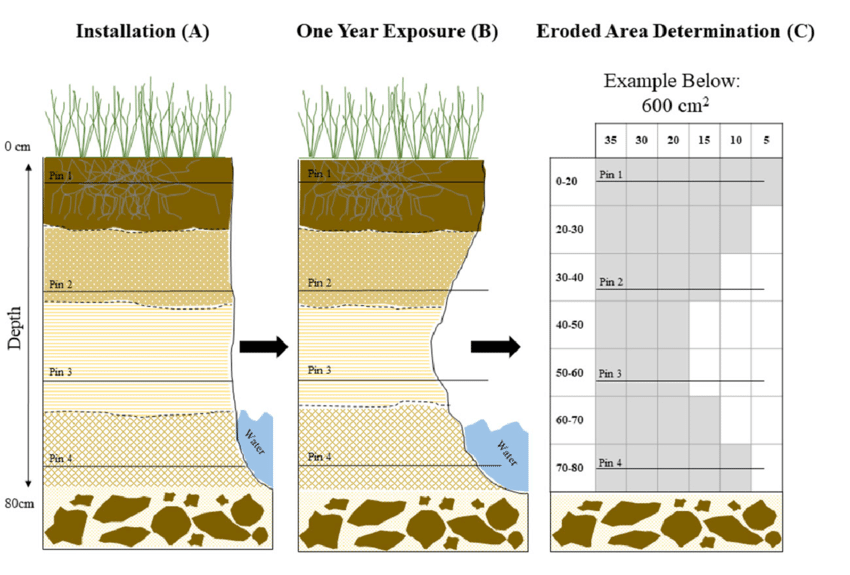
\includegraphics[width=0.5\linewidth]{figures/ch2/Erosion.png}
    \caption{Effect of Water on Bank after One Year}
    \label{fig:Effect of Water on Bank after One Year}
\end{figure}

When the combination of water level with a strong current is highest, the bank zone is affected by the tidal currents or waves. This is because, as seen in the Figure \ref{fig:Effect of Water on Bank after One Year}, water erodes the layer of the bank where the extra water level pushes, creating a dent inside the soil layer.
Consequently, after some time the upper overbank area has less and less support underneath, becoming thus unstable and partly falling down. 
Repeating this process takes the river bank further inside the land, increasing the channel width, absorbing the land near the river bank.

\newpage
\section{Hydrodynamic data}
\label{sec:Hydrodynamic data}
In this section, analysis on the hydrodynamic variables is performed. This includes relations between water elevations, discharge and sediment concentrations - through data sources as described in \ref{sec:desk study}. Additionally, tidal effects in the study area are considered. 

\subsection{Conversion to water elevation}
A uniform approach is needed to describe water levels and depths of the river. Therefore, these variables will be expressed in terms of a reference level, IGN, which is set by the \textit{Instituto Geográfico Nacional}. It is based on sea level measurements from a tide gauge in Mar del Plata, Buenos Aires province \autocite{donofrioReferenciaVertical1999}. Figure \ref{fig:waterelevationreference} gives an overview of the quantities with respect to an arbitrary measurement station. Here, $d$ is the vertical depth as measured by the ADCP or echosounder. Moreover, each station has a specific distance between its local zero reference and the zero IGN level, which is indicated by $l_{station-IGN}$. Next, all variables should be expressed in terms of IGN level. Therefore, water elevations and depths expressed in elevation are defined as follows:

\begin{equation}
    we_{station} = wl_{station} + l_{station-IGN} ~[m~IGN]
\end{equation}

\begin{equation}
    d_{el} = we_{station}-d ~[m~IGN]
\end{equation}


\begin{figure}[H]
    \centering
    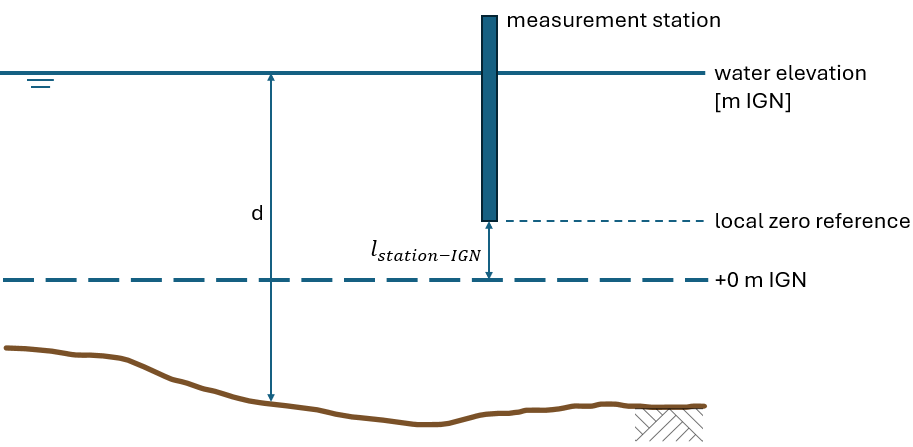
\includegraphics[width=0.75\linewidth]{figures/ch5/waterelevations.png}
    \caption{Water elevation reference}
    \label{fig:waterelevationreference}
\end{figure}

\subsection{Flow partitioning}

At some point in the Lower Paraná, the river splits into two main tributaries, as shown in Figure \ref{fig:flow partition}. To have an approximation for the distribution of discharge between these rivers, the discharge series are given in Figure \ref{fig:discharge_series}. From these plots, it follows that the majority of the discharge flows into the Paraná Guazú. Figure \ref{fig:flow_partition} represents this ratio and plots a linear fit. As there is no significant increase or decrease, the approximation is made that 78\% of the total discharge upstream of the confluence flows into Paraná Guazú. \citeauthor{reMetodologiaParaGeneracion2009} report that a linearly increasing trend occurs. In this study, more data points are used and therefore the approximation of a constant percentage is assumed sufficient. 

\begin{figure}[h!]
    \centering
    % First subfigure
    \begin{subfigure}[b]{0.48\linewidth}
        \centering
        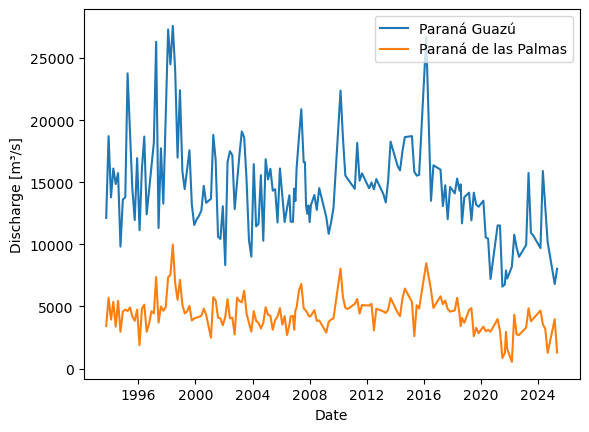
\includegraphics[width=\linewidth]{figures/ch5/discharge series.png}
        \caption{Discharge series obtained from Brazo Largo and Zárate measurement stations}
        \label{fig:discharge_series}
    \end{subfigure}
    \hfill
    % Second subfigure
    \begin{subfigure}[b]{0.48\linewidth}
        \centering
        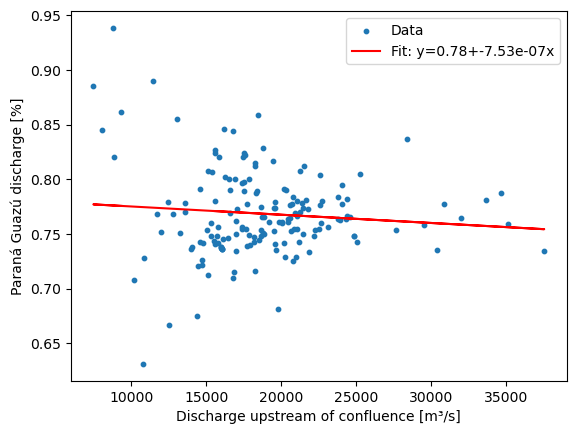
\includegraphics[width=\linewidth]{figures/ch5/flow partition.png}
        \caption{Flow partition, expressed as the share of total flow that streams into Paraná Guazú}
        \label{fig:flow_partition}
    \end{subfigure}
    
    \caption{Comparison of discharge divided between Paraná Guazú and Paraná de las Palmas}
\end{figure}



\subsection{Water elevations and discharge}
This section describes the discharge observed in the SNIH measurement stations and relates it to water elevation data. Traditionally, stage-discharge relations are described by rating curves that describe power-law dependencies between variables. This can be written in the following form, with $Q$ the discharge and $h$ the water level or stage:

\begin{equation}
\label{eq:powerlaw}
    Q = a \cdot h^b
\end{equation}

In the expression above, $a$ is a constant and $b$ an index exponent. \citeauthor{schmidtStageDischargeRelationshipOpen2011} note several limitations related to these rating curves. For example, discharge measurements typically scatter and therefore do not show a unique relation with the stage. Also, the underlying physics of the open channel are not captured in the rating. Nevertheless, the relation as given in Equation \ref{eq:powerlaw} is used to approximate dependencies between the variables. 

The relationship between fluvial discharge and water level at Brazo Largo yields a relatively weak correlation with an $R^2$ of 0.365. This is shown in Figure \ref{fig:waterleveldischarge}. Alternatively, a linear fit was assumed which produced a slightly better result, showing a positive trend with an $R^2$ of 0.444. In contrast, the El Colorado and Túnel Subfluvial stations exhibit a clear power-law dependence. Power-law fits for these stations resulted in higher $R^2$-values of 0.962 and 0.712, respectively, with the El Colorado plot shown in Figure \ref{fig:waterleveldischarge}. Overall, these results suggest that the strength of the water level–discharge relationship decreases as the river flows downstream.


\begin{figure}[h!]
    \centering

    \begin{subfigure}[t]{0.48\linewidth}
        \centering
        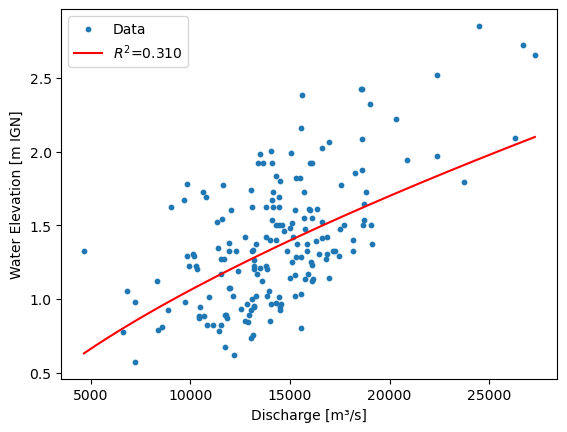
\includegraphics[width=\linewidth]{figures/ch5/wl discharge Brazo Largo.png}
        \caption{Stage–discharge relation in Brazo Largo.}
        \label{fig:wl_discharge_brazo}
    \end{subfigure}
    \hfill
    \begin{subfigure}[t]{0.48\linewidth}
        \centering
        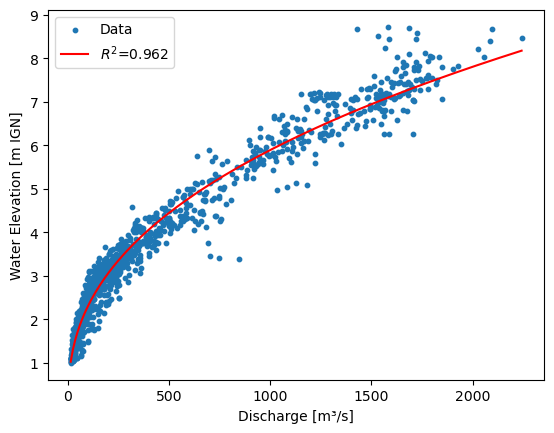
\includegraphics[width=\linewidth]{figures/ch5/wl discharge El Colorado.png}
        \caption{Stage–discharge relation in El Colorado.}
        \label{fig:wl_discharge_colorado}
    \end{subfigure}

    \caption{Water elevation–discharge relationships for two measurement stations.}
    \label{fig:waterleveldischarge}
\end{figure}



\subsection{Sediment loads}
When extending the analysis to the sediment concentrations, the same trend occurs: in the Bermejo river, fine and course sediment discharges are closely related to large flow events through power-law relations. This behaviour is found to a lesser extent in the lower Paraná, where the correlations are relatively weak. Figure \ref{fig:discharge sediment brazo} shows this relation between sediment concentrations and river discharge for the Brazo Largo station. Overall, a power-law fit seems a good approach to model the relation. The fine sediment concentration is generally higher than the course sediment concentration. In addition, the course sediment concentration increases more significantly for an increasing fluvial discharge. These are general trends, but it has to be stressed that the $R^2$ of both relationships is relatively low. As a comparison, the same variables are related for the Bermejo river in Figure \ref{fig:discharge sediment bermejo}. 


\begin{figure}[h!]
    \centering
    % First subfigure
    \begin{subfigure}[b]{0.48\linewidth}
        \centering
        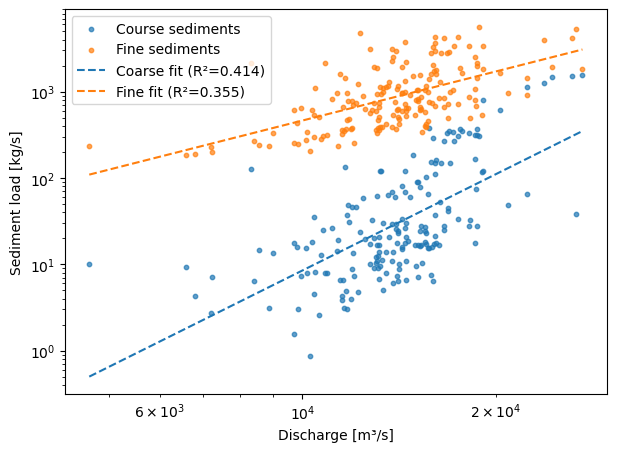
\includegraphics[width=\linewidth]{figures/ch5/discharge sediment brazo largo.png}
        \caption{Fine and course sediment loads in relation to discharge at Brazo Largo}
        \label{fig:discharge sediment brazo}
    \end{subfigure}
    \hfill
    % Second subfigure
    \begin{subfigure}[b]{0.48\linewidth}
        \centering
        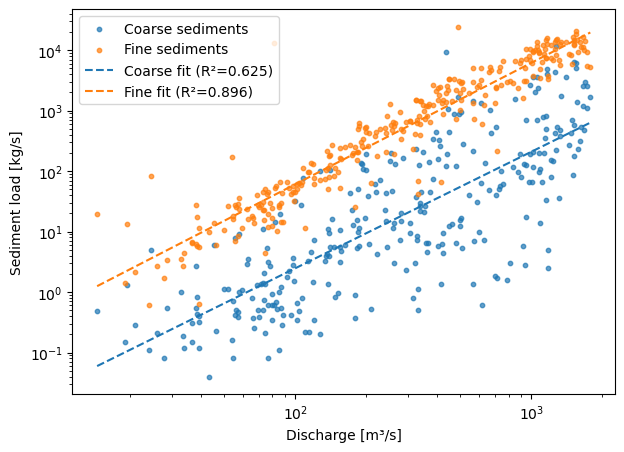
\includegraphics[width=\linewidth]{figures/ch5/discharge sediment bermejo.png}
        \caption{Fine and course sediment concentrations in relation to discharge at Bermejo}
        \label{fig:discharge sediment bermejo}
    \end{subfigure}
    
    \caption{Fine and course sediment loads related to fluvial discharge in two measurement station}
    \label{fig:sediment loads and discharge}
\end{figure}


\subsubsection{Estimated fine sediment load}
In order to study the balance of sediments in the study area, it is useful to generate time series of sediment loads. Originally intended for modelling the sedimentological dynamics of the Río de la Plata, \citeauthor{reMetodologiaParaGeneracion2009} have developed a methodology for generating time series of solid discharges. The first assumption is that the flow of solid sediments in the Middle Paraná can be represented by the sediment flows from Bermejo, disregarding the contribution of the Upper Paraná. Consequently, the flow in the Middle Paraná can be regarded as a combination of the fluvial discharge in Túnel Subfluvial and the fine sediment load recorded at El Colorado (see Section \ref{sec:measurementstations}). Next, this procedure is applied to more recent data to evaluate the methodology. The most recent, relevantly long interval with continuous data for both measurement stations is 2017 to 2019. A number of assumptions is used to find the time series of fine sediment concentration:

\begin{itemize}
    \item A base concentration is set for the Middle Paraná to compensate for low inflow periods of the Bermejo. Therefore, fine sediment load data from Itatí and Puerto Pilcomayo stations (SNIH) are studied in the relevant interval. The sum of the mean loads gives a base concentration of $182.96$ kg/s.
    \item To cover for the distance between El Colorado and Túnel Subfluvial, a delay of 222 hours is considered (approximately 800 km at a flow velocity of 1 m/s). 
    \item Depositions of wash load in the floodplain between the stations, is compensated for by substracting 10 million tonnes per year from concentration peaks. This holds for all concentrations above a certain threshold value, which in this case was found to be optimal at $350$ mg/l.
\end{itemize}

The result of this time series is given in Figure \ref{fig:timeseries fine sediments}. It is important to note that this relation for fine sediment concentrations is considered useful for the Paraná Guazú as well \autocite{reMetodologiaParaGeneracion2009}. The plot shows that the observations are generally higher than the fit predicts in times of low fine sediment loads. Overall, the fit gives a good estimate of fine sediment concentrations, revealing seasonal aspects and relevant concentration values.

\begin{figure}[H]
    \centering
    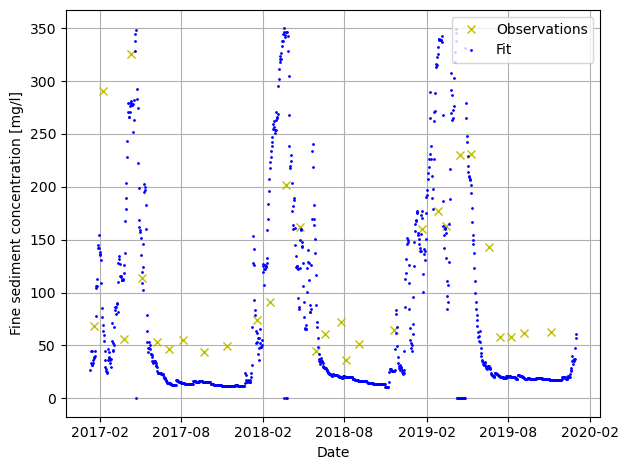
\includegraphics[width=0.5\linewidth]{figures/ch6/fine sediment concentrations.png}
    \caption{Fine sediment concentration time series}
    \label{fig:timeseries fine sediments}
\end{figure}



\subsubsection{Estimated coarse sediment load}
An approach for estimating the transport of coarse sediments is based on the Engelund–Hansen formulation (\cite{engelundMonographSedimentTransport1967}). This empirical relation predicts the total transport of bed material, which in this case is assumed to consist mainly of coarse sediments or sands. The total volumetric sediment transport rate per unit width is expressed as:

\begin{equation}
    q_{t} = \frac{0.05\,u^{2}\,h^{3/2}\,S_{f}^{3/2}}{(s - 1)^{2}\,g^{1/2}\,d_{50}}
    \label{eq:engelund_hansen}
\end{equation}

where \( s \) is the specific gravity of the sediment, \( g \) is the acceleration due to gravity, \( d_{50} \) is the median grain diameter, and \( S_{f} \) is the friction slope. The variables \( u \) and \( h \) represent the mean flow velocity and the flow depth, respectively. The value for $d_{50}$ is assumed to be $200 ~\mu m$ \autocite{reMetodologiaParaGeneracion2009}. The values for $u$, $h$ and $S_f$ were gathered by running a one-dimensional hydrodynamic model in HEC-RAS. 





\subsection{Correlation between variables}
\label{sec:correlation of variables}
The approach of defining the relations between measured flow variables is as follows. First, the values in the dataset are log-transformed, after which $R^2$-values are calculated based on a linear fit on the logarithmic values. This procedure is applied to the variables of all measurement stations as described in Section \ref{sec:measurementstations}. Figure \ref{fig:correlationmatrices} gives the results for El Colorado and Brazo Largo in the form of correlation matrices. It stands out that correlations in the Bermejo are very high for all variables. This indicates that the power-law assumption is suitable for describing the dependencies between these variables. Subsequently, it is found that correlations for the Brazo Largo are much smaller. This is also the case for the Zárate station on the Paraná de las Palmas. As this river is also located in the Lower Paraná, this behaviour is expected. 

Analysis of the flow variables has shown that $R^2$-values tend to decrease, the further downstream the location of the measurements is. This result is in agreement with those found by \citeauthor{songEvaluatingUnderstandingTideriver2024}, who state that the stage-discharge relationship is considerably affected in the transitional zone and tide-dominated region of the Yangtze estuary. Their research reports $R^2$-values decreasing from 0.9 to 0.4, in a river-dominated and transitional zone, respectively. Therefore, an in-depth study of the tide-river interactions is needed. This includes measurements in both the transitional zone and tide-dominated region, to update the stage-discharge relationship. For this particular study, the influence of tidal effects are handled in Section \ref{sec:tidal forcing}.

As for the sediment-discharge relationship, the differences in correlations in Brazo Largo can be explained through the sources of the variables. Whereas the fine sediment concentration predominantly originates from the Bermejo basin, the discharge is dominated by the Paraguay and Paraná. This results in a weak correlation downstream of the confluence of these rivers \autocite{lopezweibelSourcesTemporalDynamics2022}. Another factor that may perturb the correlation of variables in the Lower Paraná, is the inflow of the Uruguay river. The variation in elevations that occur due to the presence of this river, can cause disturbances in the rating curves. 


\begin{figure}[h!]
    \centering
    % First subfigure
    \begin{subfigure}[b]{0.48\linewidth}
        \centering        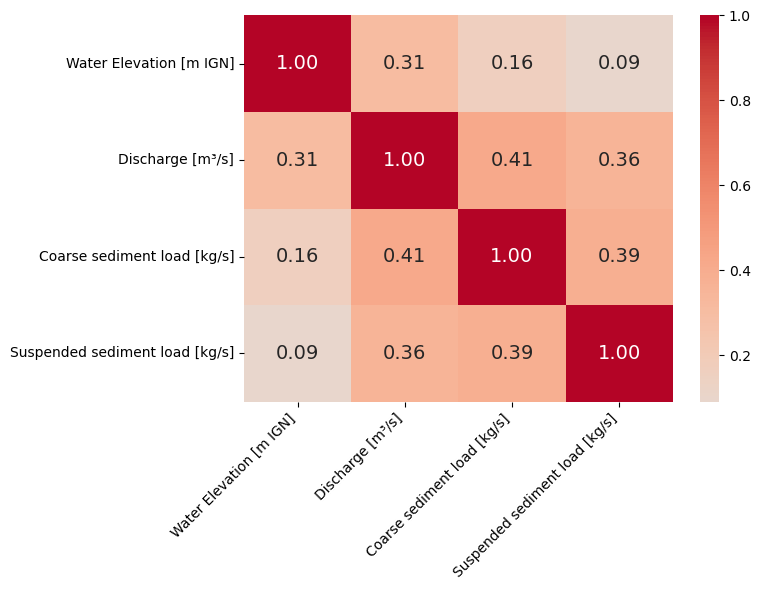
\includegraphics[width=\linewidth]{figures/ch5/logcorrelations Brazo Largo.png}
        \caption{Correlation matrix of log-transformed data in Brazo Largo}
        \label{fig:logcorrelation brazo}
    \end{subfigure}
    \hfill
    % Second subfigure
    \begin{subfigure}[b]{0.48\linewidth}
        \centering
        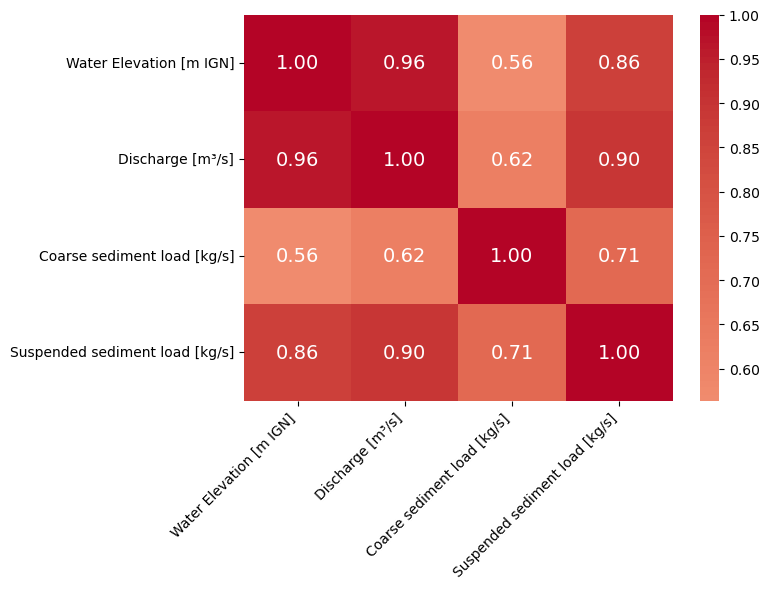
\includegraphics[width=\linewidth]{figures/ch5/logcorrelations Bermejo.png}
        \caption{Correlation matrix of log-transformed data in El Colorado}
        \label{fig:logcorrelation bermejo}
    \end{subfigure}
    
    \caption{Comparison of $R^2$-values at Brazo Largo and El Colorado}
    \label{fig:correlationmatrices}
\end{figure}




\subsection{Tidal forcing (Values are incorrect, has to be changed)}
\label{sec:tidal forcing}
The tidal wave of the Atlantic Ocean influences the hydrodynamics of the lower Paraná delta. As the tidal wave enters the delta at the Río de la Plata, the tide is damped and phased by friction, channel geometry and branching, resulting in a reduced amplitude and an increase in phase delay. Under normal conditions, the influence of the tide on the Paraná River reaches the city of Villa Constitución, which is located 220 km upstream of the river mouth. For storm conditions, the tide can reach the city of Rosario \autocite{balayCausesPeriodicityLarge2018}. In order to determine the influence of the tide at Brazo Largo, a harmonic tidal analysis is performed on hourly water level measurements. This analysis consists of decomposing the observed water level time series into a sum of sinusoidal components, with each of these components representing a specific tidal constituent. The tidal constituents considered for Brazo Largo are shown in Table \ref{tab: constituents}.

\begin{table}[H]
\centering
\caption{Tidal constituents used to reconstruct the tide
\autocite{apelPrinciplesOceanPhysics1987}.}
\label{tab: constituents}
\begin{tabular}{lccc}
\hline
Tidal constituent & Name & Period [h] \\
\hline
\multicolumn{3}{l}{\textit{Semi-diurnal}} \\
\hspace{1em}Principal lunar & M2 & 12.4206\\
\hspace{1em}Principal solar & S2 & 12.0000 \\
\hspace{1em}Lunar elliptical & N2 & 12.6583\\
\hline
\multicolumn{3}{l}{\textit{Diurnal}} \\
\hspace{1em}Lunar-solar declinational & K1 & 23.9345  \\
\hspace{1em}Principal lunar & O1 & 25.8193  \\
\hline
\multicolumn{3}{l}{\textit{Shallow water constituents}} \\
\hspace{1em}Overtide of M2 (quarter-diurnal) & M4 & 6.2103  \\
\hline
\end{tabular}
\end{table}



\begin{table}[H]
\centering
\setlength{\tabcolsep}{8pt} 
\caption{Computed amplitude and phase}
\begin{tabular}{lcccccc}
\hline
Constituent & $A_{\text{BL}}$ & $\phi_{\text{BL}}$ [$^\circ$] \\
\hline
M2 & 0.0764 & 338.51 \\
S2 & 0.0116 & 82.10 \\
N2 & 0.0284 & 0.022 \\
K1 & 0.0331 & 299.3  \\
O1 & 0.0672 & 0.061 \\
M4 & 0.0085 & 0.006  \\
\hline
\end{tabular}
\end{table}

Figure 5.7 shows the water level time series for a period of 7 days compared to the calculated tidal signal at Brazo Largo. From this figure, it can be seen that the measured water level follows the same tidal oscillations. However, the tide does not explain all the variability of the water level; the measured water level also shows large variability caused by discharge and wind. 
\\The influence of the strong non-tidal component is confirmed by Figure 5.8, which shows the water level at Brazo Largo for a period of 2 years. The measured water level fluctuates greatly, reaching +2.0 m and -0.5 m while the tidal component is steady at 0.0 m with an amplitude of 0.17 m. The tidal forcing is relatively small compared to the river and seasonal influences. Tidal forcing is therefore subordinate to other forcings such as discharge.

\begin{figure}[H]
    \centering
    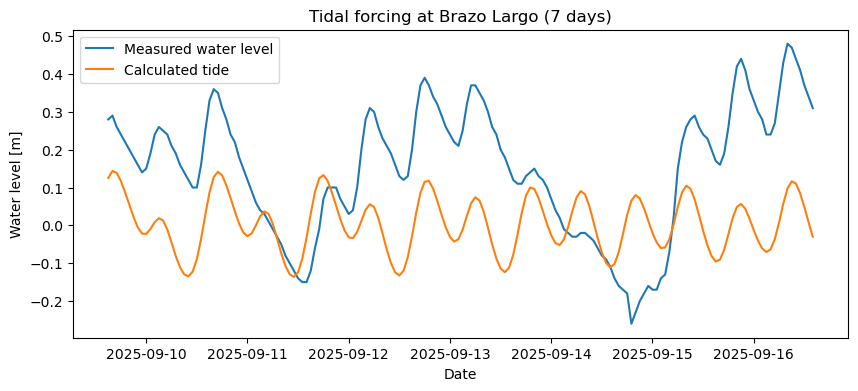
\includegraphics[width=1\linewidth]{figures/ch5/Tide_Brazo_largo.png}
    \caption{Calculated tide at Brazo Largo for a period of 7 days.}
    \label{fig:period 7}
\end{figure}
\begin{figure}[H]
    \centering
    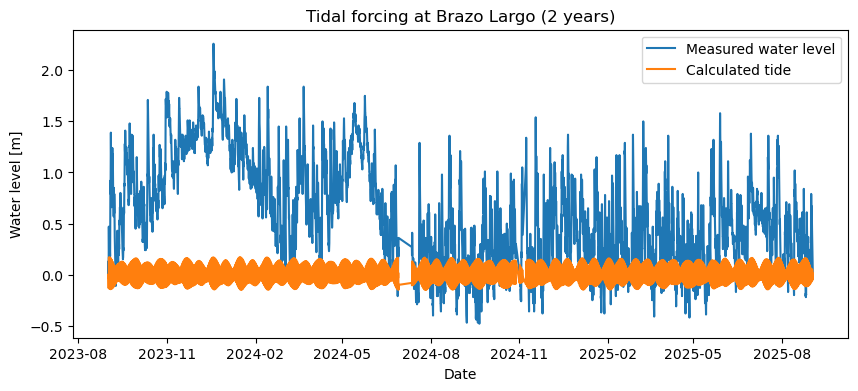
\includegraphics[width=1\linewidth]{figures/ch5/Tide_BL_2y.png}
    \caption{Calculated tide at Brazo Largo for a period of 2 years.}
    \label{fig:period 2}
\end{figure}



\newpage
\section{Field work measurements}
This section describes the results of the field campaign introduced in Section \ref{sec:field study}. The measurements are compared to the results found in Section \ref{sec:Hydrodynamic data}.


\subsection{Water level and discharge}
In order to further study the liquid flows in the Paraná Guazú, estimates are needed for the discharge of Río Ibicuy and Río Talabera. These were collected during the fieldwork, as indicated in Figure \ref{fig:measurements day1} and Figure \ref{fig:measurements day2}. In addition, an overview of all cross sections with discharge measurements is given in Figure \ref{fig:cross section domain}. The indexing of the cross sections is made in chronological order based on the fieldwork. Note that at the confluence of the Ibicuy and Paraná, there is no measurement of the component flowing in from the Paraná. However, this can be estimated by the equilibrium of discharges in the confluence. 

\begin{figure}[H]
    \centering
    \includegraphics[width=0.75\linewidth]{figures/ch5/balance domain.png}
    \caption{Overview of cross sections with discharge measurements}
    \label{fig:cross section domain}
\end{figure}

The relevant flow measurements of the different cross sections are summarized in Table \ref{tab:discharges fieldwork}. Note that the water levels are recorded on different dates from nearby measurement stations, i.e. Brazo Largo and Ibicuy. Figure \ref{fig:water elevations fieldwork} gives an overview of the evolution of water elevations during the measurement campaign. The values in the table correspond to the location and time of each measurement. For Section 5, the water level is linearly interpolated between the stations. The remaining cross sections are assumed to be close enough to their corresponding measurement station.  Also, the flow velocity is a mean velocity taken over the entire cross section of the two measured sections per measurement location. The bathymetries and velocity profiles that result from the ACDP measurements can be found in Appendix \ref{appendix:fieldwork results}, where the output of the \textit{RiverSurveyor} software is given. Note that of each cross section, only one of the two measured sections is given. 

\begin{table}[H]
    \centering
    \renewcommand{\arraystretch}{1.2} % extra row spacing
    \setlength{\tabcolsep}{8pt}       % extra column spacing
    \caption{Flow properties of fieldwork measurements in different sections}
    \begin{tabular}{llccc}
        \toprule
        Section & River & Water level [m IGN] & Mean flow velocity [m/s] & Discharge [$m^3$/s] \\
        \midrule
        1 & Talabera       & 1.09 & 0.619 & 4402 \\
        2 & Paraná Guazú   & 1.12 & 0.507 & 6562 \\
        3 & Paraná Guazú   & 1.10 & 0.573 & 10748 \\
        \midrule
        4 & Ibicuy & 0.87 & 0.445 & 2901 \\
        5 & Paraná Guazú   & 0.82 & 0.566 & 6758 \\
        \bottomrule
    \end{tabular}
    \label{tab:discharges fieldwork}
\end{table}

\begin{figure}
    \centering
    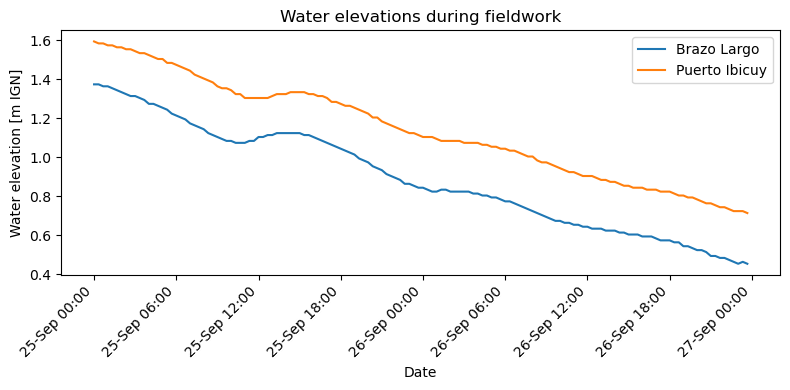
\includegraphics[width=0.75\linewidth]{figures/ch6/water elevations fieldwork.png}
    \caption{Water elevations of Brazo Largo and Puerto Ibicuy during fieldwork}
    \label{fig:water elevations fieldwork}
\end{figure}

The water elevations in Figure \ref{fig:water elevations fieldwork} are expressed with respect to the IGN datum. For that reason, elevations at Puerto Ibicuy are consistently higher than at Brazo Largo on the same time instants. During the two measurement days, water levels drop while discharges increase, which appears to contradict the positive correlation between stage and discharge discussed in Section \ref{sec:correlation of variables}. This discrepancy arises because the standard stage-discharge relationship assumes steady flow and acts on longer timescales. In contrast, on short timescales, water levels in the Paraná Guazú are influenced by variations in the Río de la Plata, including backwater effects and transient downstream control. These factors cause a temporary inverse relation between stage and discharge, leading to the observed short-term response. \citeauthor{jonesExpandedRatingCurve2019} confirm that traditional rating curves fail in the tidal zone, because tidally influenced discharge is more complex than upstream river discharge, causing non-monotonic behaviour. 




\subsection{Grain size distribution of bed load samples}
\label{sec:grainsizedistribution}
During the fieldwork, data was collected on the Paraná River over a period of two days. Seven samples were collected from the riverbed at four different cross-sections. Samples were collected at depths of 10 and 15 metres. The identification numbers of each sample are determined as follows. The first number refers to the location of the cross-section, and the second number refers to a depth of 10 or 15 metres. The locations where the samples were collected are presented in Figure \ref{fig:measurements day1} and \ref{fig:measurements day2}. Sample 3-1 was quite large, so it was decided to treat it as two different samples (3-1A \& 3-1B). 

When processing the samples, it was decided to start with a 0.5 mm sieve size for the samples that appeared to be sand and a 0.354 mm sieve size for the other samples. This was done because only six sieves and one residue container fit into the sieving setup. After sieving the samples for 10 minutes, each quantity of sample per sieve was weighed. This was used to calculate a cumulative grain size distribution. The calculation and processing of the results are  described in more detail in Appendix \ref{appendix:Lab data}. The results are presented in Figure \ref{fig:Cumu}.


\begin{figure}[H]
    \centering
    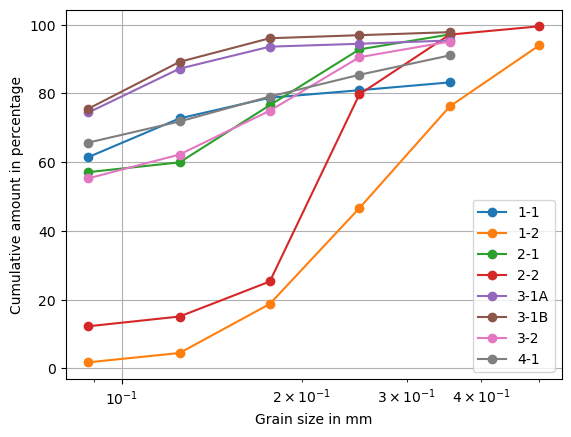
\includegraphics[width=0.75\linewidth]{figures//ch6/CUMU.png}
    \caption{Cumulative grain size distribution of bed load samples}
    \label{fig:Cumu}
\end{figure}

Figure \ref{fig:Cumu} clearly shows that 1-2 and 2-2 are sand samples and the other samples are clay and silt samples. During the test, possible organic materials were also looked at. When seeing something that could be organic, the sample was tested with hydrochloric acid to see if this was the case. However, no organic particles have been found in the samples. 

From Figure \ref{fig:Cumu}, it can be seen that sand is more frequently encountered at 15 m depth than at 10 m depth. This suggests that coarser sediments tend to occur in the deeper parts of the channel, which are typically subject to stronger flow and higher bed shear stresses. Since there are no sediment samples available in the study area, this cannot be validated directly. Nevertheless, INA has recently recovered multiple samples in the river near the city of Rosario. Two of those samples were taken at a depth of 30 meters. These are presented in Figure \ref{fig:rd}, Together with the Paraná Guazú sand samples and a grain size distribution of Ottawa fracking sand. As can be read in Section \ref{sec: fracking in argentina}, the demand of fracking is increasing through the years, rising the question if river sand can also be used for these practices.
That's why some data about fracking sand from Section \ref{sec:Charact. of fs} is combined with the gained data in this Section. 

\begin{figure}[H]
    \centering
    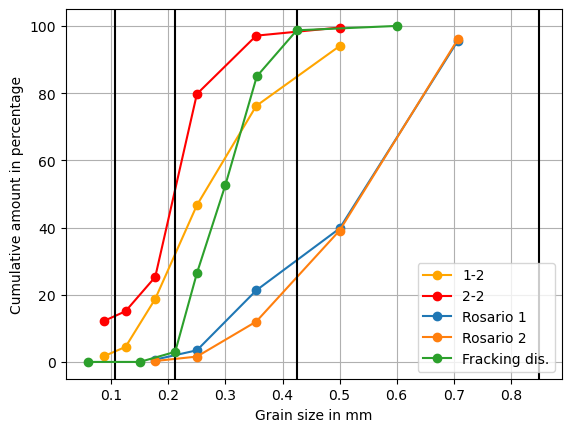
\includegraphics[width=0.75\linewidth]{figures//ch6/comparison2.png}
    \caption{CGZD of multiple samples with homogneneous demand lines \autocite{bensonFracSandUnited2015}}
    \label{fig:rd}
\end{figure}

As can be seen from Figure \ref{fig:rd}, the average particle size of the sand tends to increase with recovery depth. This pattern likely reflects natural sediment sorting processes, where finer particles are carried further by the current, while coarser grains settle in deeper or higher-energy parts of the channel. Such a trend is consistent, yet it should not be assumed to hold universally across all river systems.

It is important to emphasize that the data supporting this observation were collected outside the river section that falls within the area of interest. Consequently, before drawing any conclusions, it is essential to conduct targeted sampling and grain size analysis within the study area. Only by verifying these local conditions, it can be confirmed whether the same coarsening trend applies here as well.

When these findings are related to the requirements for sand used in hydraulic fracturing (fracking), it becomes apparent that even with the observed increase in grain size, the river sand does not meet the necessary specifications. Fracking sand requires a very uniform grain size distribution to ensure consistent permeability and mechanical strength within the proppant pack. At least 90\% of the particle sizes must fall within a defined size range, represented by the black boundary lines in the accompanying figure \autocite{bensonFracSandUnited2015}.
Furthermore, this acceptable range tends to widen as the target grain size increases, reflecting a broader tolerance for larger particles. However, the natural river sands under consideration display too much variability in grain size to be classified as suitable fracking sand without additional processing or sieving.


\subsection{Suspended sediment load}
\label{sec: Suspended sediment load}
In this section, the measured suspended sediment concentrations and flow velocity profiles are analysed in order to calculate the total suspended sediment flux. The sediment concentrations were obtained by lowering an intake tube connected to a rope and a weight into the water, as described in Section \ref{Measurement variables and equipment}. By assuming a constant angle of the rope at different depths in a cross section and measuring the length of the rope, the depth at which the measurements were taken could be determined. The measured suspended sediment concentrations at different depths are shown in Figure \ref{fig:Measured suspended sediment concentrations}.

\begin{figure}[H]
    \centering
    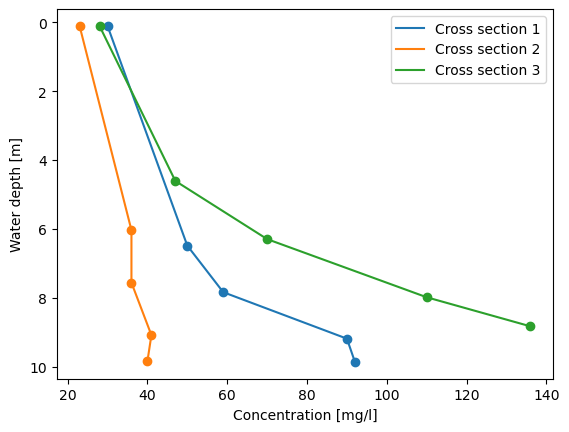
\includegraphics[width=0.75\linewidth]{figures/ch6/Measured_SSC.png}
    \caption{Measured suspended sediment concentrations.}
    \label{fig:Measured suspended sediment concentrations}
\end{figure}

Figure \ref{fig:Measured suspended sediment concentrations} shows, that for all three cross sections, the suspended sediment concentration is the highest near the bed, which is typical for suspended sediment. The steeper profile for cross section 2 higher turbulence or finer particles compared to cross sections 1 and 3. Higher turbulence combined with finer particles causes sediment to stay suspended more easily, which results in a steeper concentration gradient with depth.

The Acoustic Doppler Current Profiler (ADCP) measures the flow velocity and depth across a river cross section by dividing the measurements into vertical bins for every ensemble. These data can be used to create a flow velocity field for the whole cross section, see Appendix \ref{appendix:fieldwork results}, and velocity profiles for every ensemble along the cross section. These velocity profiles are used to determine the Law of the Wall fit, see Equation \ref{eq:law_of_the_wall}.

\begin{equation}
    u = \left( \frac{u_*}{\kappa} \right) \ln\left( \frac{z}{z_0} \right)
    \label{eq:law_of_the_wall}
\end{equation}

The Law of the Wall describes the velocity profile of a turbulent flow near a boundary. Therefore, the log-law is fitted on only the velocity points in the lowest 50\% of the water column. Additionally, the Law of the Wall is used to calculate the shear velocity ($u_*$), which is most accuratly determined from the near-bed region. By fitting only on the lower 50\%, the fit is not affected by upper flow deviations such as wind, waves and secondary flow. 

The measured flow velocity profiles by the ADCP and the fitted Law of the Wall are shown in Figure \ref{fig: Velocity profiles cross sections} for the three locations of the concentration measurements. The mean flow velocities for cross sections 1 and 2 are very similar, whereas Cross Section 3 shows a slightly higher mean velocity. This increased flow velocity can be explained by flow concentration as a result of the nearby confluence.

\begin{figure}[H]
    \centering
    \begin{subfigure}[b]{0.31\linewidth}
        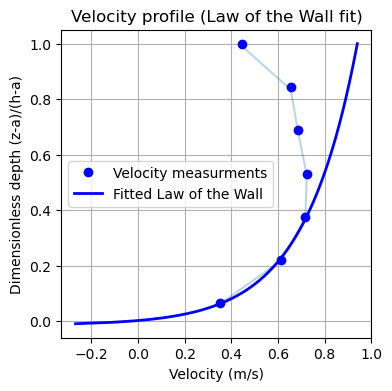
\includegraphics[width=\linewidth]{figures/ch6/cs1_vel_profile.png}
        \caption{Cross section 1.}
    \end{subfigure}
    \hfill
    \begin{subfigure}[b]{0.31\linewidth}
        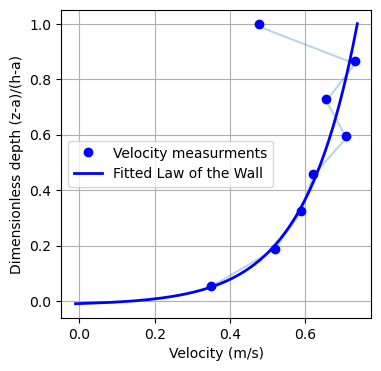
\includegraphics[width=\linewidth]{figures/ch6/cs2_vel_profile.png}
        \caption{Cross section 2.}
    \end{subfigure}
    \hfill
    \begin{subfigure}[b]{0.31\linewidth}
        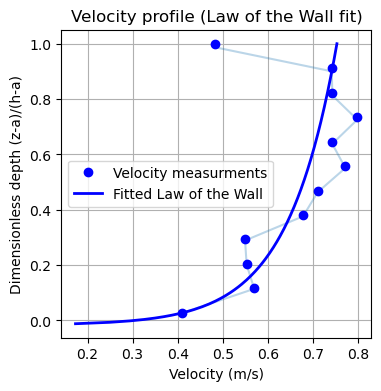
\includegraphics[width=\linewidth]{figures/ch6/cs3_vel_profile.png}
        \caption{Cross section 3.}
    \end{subfigure}
    \caption{Velocity profiles with Law of the Wall fit for the three cross sections.}
    \label{fig: Velocity profiles cross sections}
\end{figure}


The computed shear velocity ($u_*$) from the Law of the Wall fit is used to calculate the Rouse number at every ensemble along the cross section; see Equation \ref{Rouse number}. Using this Rouse number it is possible to calculate the sediment concentration ($c$) at any depth ($z$) in the water column using the Rouse profile in Equation \ref{Rouse profile}.

\begin{equation}
    P = \frac{w_s}{\kappa u_*}
    \label{Rouse number}
\end{equation}

\begin{equation}
    \frac{C}{C_a} = \left( \frac{z - z_0}{a - z_0} \cdot \frac{h - a}{h - z} \right)^{P}
    \label{Rouse profile}
\end{equation}

The reference depth ($a$) and the near-bed reference concentration ($C_a$) were based on the lowest suspended sediment concentrations measured for each cross section. By inspecting the Rouse profile at the ensemble where the sediment measurements were taken, the settling velocity ($w_s$) was determined, as no information on suspended sediment size was available. The Rouse profile for the location at which the suspended sediment measurement in cross section is shown in Figure \ref{fig:RouseProfile_cs11}. The corresponding velocity profile and Law of the Wall fit are shown in \ref{fig:Vel_profile_cs11}. The velocity profile measurements show a decreased velocity near the water surface, likely due to wind effects, proving why it is important to fit only on the lowest 50\% of the depth.

\begin{figure}[H]
    \centering
    \begin{minipage}[b]{0.48\linewidth}
        \centering
        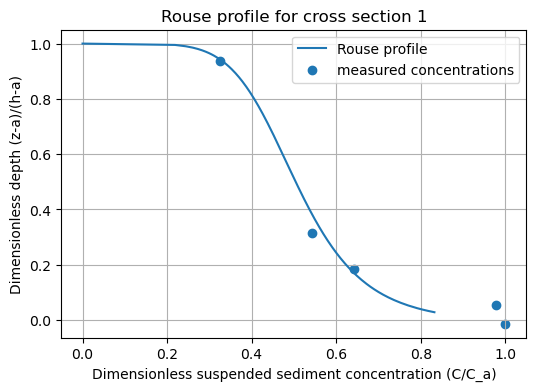
\includegraphics[height=6cm]{figures/ch6/RouseProfile_cs11.png}
        \caption{Rouse profile for Cross section 1.}
        \label{fig:RouseProfile_cs11}
    \end{minipage}
    \hfill
    \begin{minipage}[b]{0.48\linewidth}
        \centering
        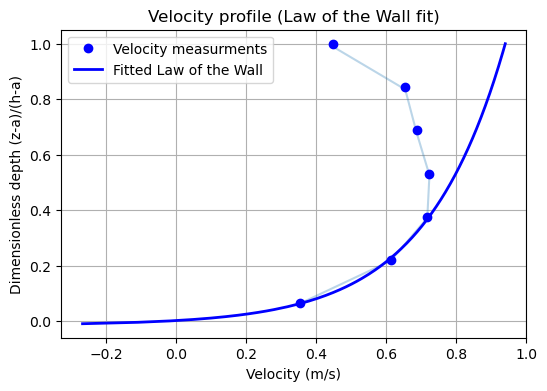
\includegraphics[height=6cm]{figures/ch6/cs1_vel_big.png}
        \caption{Velocity profile for Cross section 1.}
        \label{fig:VelProfile_cs11}
    \end{minipage}
\end{figure}

As stated above, the settling velocity is determined by fitting the Rouse profile to the measured concentrations. 
The estimated settling velocities are shown in Table~\ref{tab: Overview settling velocity} for the three cross sections. 
Additionally, the corresponding sediment grain diameter is given, which is calculated using the Ferguson and Church \autocite{fergusonSimpleUniversalEquation2004} formula (Eq.~\ref{eq: Settling vel formula}). The surbmerged specific density ($R$) is 1.65 for quartz in water and the kinematic viscosity ($\nu$) of the fluid is 1.0 $\times 10^{-6}~\ \text{m}^2\text{/s}$ for water at 20~\textdegree C. The empirical shape coefficients $C_1$ and $C_2$ which reflect viscous and turbulent drag and have a value of 18 and 0.4 respectively.

\begin{equation}
    w_s = \frac{R g d^2}{C_1 \nu + \sqrt{0.75\, C_2\, R g d^3}}
    \label{eq: Settling vel formula}
\end{equation}

The lower settling velocity and thus the lower particle diameter for cross section 2, in Table \ref{tab: Overview settling velocity}, corresponds to the steeper gradient of sediment concentration in Figure \ref{fig:Measured suspended sediment concentrations}. The computed grain diameters all fall within the range of silt.  

\begin{table}[H]
    \centering
    \caption{Estimated settling velocities ($w_s$) with diameter ($d$) per cross section}
    \label{tab: Overview settling velocity}
    \setlength{\tabcolsep}{8pt}
    \begin{tabular}{c c c}
        \hline
        Cross Section & $w_s~[m/s]$ & $d~[mm]$  \\
        \hline
        1 & 0.0015 &  0.042 \\
        2 & 0.00035  &  0.020 \\
        3 & 0.0025 & 0.054 \\
        \hline
    \end{tabular}
\end{table}

The suspended sediment flux per cross section is calculated by first multiplying the concentration at any given depth, from the Rouse profile, with the corresponding velocity and a depth increment; see Equation \ref{eq: sediment flux formula}. This flux per unit width is multiplied by the ensemble width to get the ensemble sediment flux for every point along the cross section. 

\begin{equation}
    q_{s} = \int_{a}^{h} C(z, \alpha C_a) \, u(z) \, dz
    \label{eq: sediment flux formula}
\end{equation}

The total suspended sediment flux for every cross section is calculated by summing the ensemble fluxes. These calculated total suspended fluxes in kg/s are displayed in Table \ref{tab:Calculated suspended sediment flux}. For every cross section two different ADCP measurements were taken. The table shows the computed suspended sediment flux based on the velocity profiles of these two tracks and the mean suspended sediment flux for the three cross sections. This mean flux is the value that will be used to set up the sediment balance in Section \ref{sec: Sediment Balance}. 
 
\begin{table}[H]
    \centering
    \caption{Calculated suspended sediment fluxes at different cross sections (kg/s)}
    \label{tab:Calculated suspended sediment flux}
    \setlength{\tabcolsep}{8pt}
    \begin{tabular}{c c c c}
        \hline
        Cross Section & Track 1 & Track 2 & Mean\\
        \hline
        1 & 127.14 & 115.61 & 121.38\\
        2 & 90.80  & 61.54  & 76.17\\
        3 & 337.44 & 348.07 & 342.76\\
        \hline
    \end{tabular}
\end{table}

\textbf{Uncertainties} \\
The calculation of the suspended sediment flux is subject to several sources of uncertainty. Firstly, for each cross section, suspended sediment concentration was measured at only one location. Because no information is available on the grain size distribution, the settling velocity ($w_s$) for the entire cross section was determined by calibrating the Rouse profile to fit this single measurement. Consequently, instead of calculating a separate Rouse profile for each grain size bin, the calibrated $w_s$ was assumed to be representative for all sediment grains across the cross section. The lack of grain size information and the assumption of a representative $w_s$ introduce considerable uncertainty into the results.

Secondly, after plotting the depth averaged velocities along the three cross sections, it was found that the velocities show a spread of $\pm0.2~m/s$. The average flow velocity for the three cross sections is around $0.5-0.6~m/s$, see Table \ref{tab:discharges fieldwork}. As the suspended sediment flux is calculated by multiplying the concentration by the velocity, this uncertainty in velocity (approximately $30-40\%$ of the mean flow) can lead to a comparable relative uncertainty in the calculated suspended sediment flux. In addition, part of the uncertainty may come from short-term flow fluctuations during the measurements and from spatial variability within the cross section that is not fully captured by the ADCP transects.

To assess the reliability of the measurement concentrations, the estimations are compared to the existing relationship between fine sediment loads and fluvial discharge in Brazo Largo. Figure \ref{fig:fine measurements} shows the measurements conducted around the confluence. It stands out that discharges are quite small, while the loads of section 1 and section 3 are close to the fit. The fine sediment load measured in section 2 is relatively low. This is possibly an underestimation of the real inflow into the confluence, which might affect the sediment balance. 


\begin{figure}[h!]
    \centering
    % First subfigure
    \begin{subfigure}[b]{0.48\linewidth}
        \centering        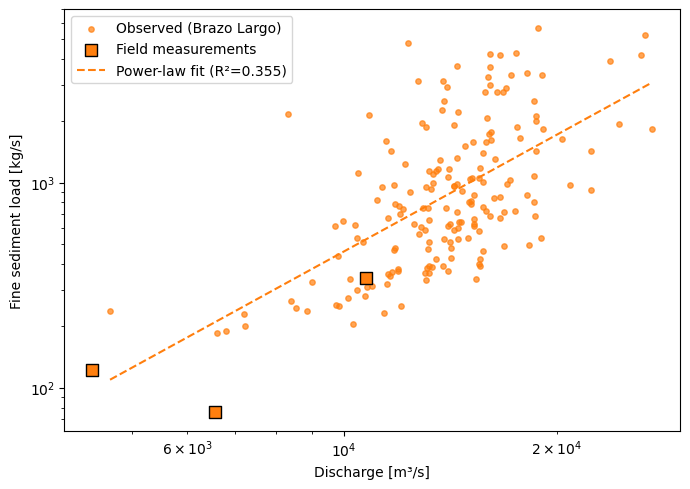
\includegraphics[width=\linewidth]{figures/ch6/fine measurements.png}
        \caption{Fine sediment load - discharge relation for Brazo Largo including estimations based on field data}
        \label{fig:fine measurements}
    \end{subfigure}
    \hfill
    % Second subfigure
    \begin{subfigure}[b]{0.48\linewidth}
        \centering
        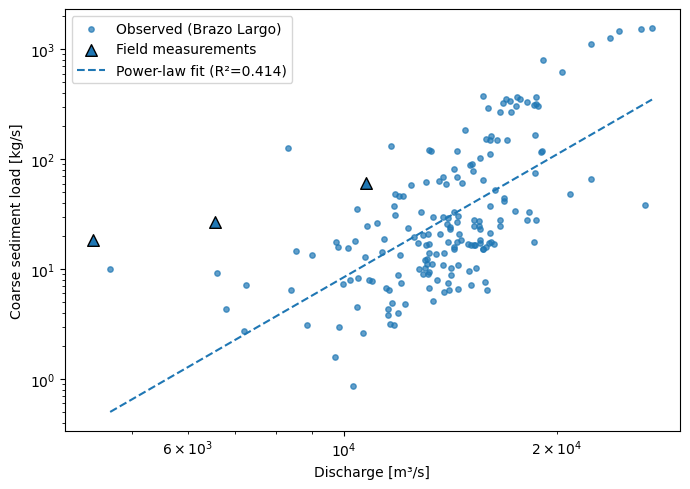
\includegraphics[width=\linewidth]{figures/ch6/course measurements.png}
        \caption{Course sediment load - discharge relation for Brazo Largo including estimations based on field data }
        \label{fig:course measurements}
    \end{subfigure}
    
    \caption{Comparison of estimations based on field measurements to historical data of sediment loads}
    \label{fig:correlationmatrices}
\end{figure}

\subsection{Bed load}
\label{sec: Bed load}
This section presents estimates of the total bed load, based on the grain size distribution of the bed samples described in Section \ref{sec:grainsizedistribution}. Most samples consisted of clays and silts, while two were classified as sand. This distinction strongly depends on the recovery depth of the bed samples. Considering the variability in bed material composition, a careful selection of the model used to estimate bed load transport is required. 

Because the Engelund–Hansen formula was derived for non-cohesive sand-bed conditions, it is only applied to the samples identified as sand (\cite{engelundMonographSedimentTransport1967}). The remaining samples, consisting of clays and silts, are cohesive and therefore not suitable for estimation with this method. The formula is repeated here for clarity:

\begin{equation}
    q_{t} = \frac{0.05\,u^{2}\,h^{3/2}\,S_{f}^{3/2}}{(s - 1)^{2}\,g^{1/2}\,d_{50}}
    \label{eq:engelund_hansen}
\end{equation}

In which:
\begin{itemize}
    \item $u$ ~[m/s]: mean flow velocity in cross section (see Table \ref{tab:discharges fieldwork})
    \item $h$ ~[m]: mean flow depth
    \item $S_f = 10^{-5}$: friction slope, approximated here as the bed slope (\cite{lopezweibelSourcesTemporalDynamics2022})
    \item $s = 2.65 ~[-]$: specific gravity
    \item $d_{50}$ ~[$\mu$m]: mean grain size, derived from grain size distribution through linear interpolation
\end{itemize}

Using a channel width $B$ and a volumetric weight of $\rho_s = 2650 $ kg/m$^3$, the total mass transport can then be expressed as follows:

\begin{equation}
    Q_b = q_t \cdot B \cdot \rho_s
 \end{equation}

 Table \ref{tab:engelund-hansen} performs the calculation using the corresponding input parameters for section 1, 2 and 3 respectively. Note that for section 3, a value for $d_{50}$ is assumed because the grain size distribution showed that the sample taken at a depth of 15 meters did not contain sand. 


\begin{table}[H]
    \centering
    \renewcommand{\arraystretch}{1.2} % extra row spacing
    \setlength{\tabcolsep}{8pt}       % extra column spacing
    \caption{Engelund--Hansen input parameters and total bed load}
    \begin{tabular}{lcccc}
        \toprule
        Section & $B$ [m] & $h$ [m]
         & $d_{50}$ [\textmu m]
         & $Q_b$ [kg/s]\\
        \midrule
        1 & 544 & 13.04 & 262 & 18.43 \\
        2 & 917 & 13.36 & 210 & 26.92 \\
        3 & 932 & 18.60 & 200 & 60.32 \\
        \bottomrule
    \end{tabular}
    \label{tab:engelund-hansen}
\end{table}

\subsubsection{Uncertainties}
The uncertainties in estimating bed load transport are primarily related to the composition of the bed material. Engelund-Hansen is used here, which is predominantly suited for sandy beds. As observed during field measurements, the Paraná Guazú contains significant amounts of fine sediments, such as clays and silts. In some samples, no sand was detected; however, this largely depended on the sampling depth—at deeper locations, sand was indeed present. Therefore, the application of Engelund-Hansen is justified, and it can be assumed that section 3 also contains sand. The sediment diameter is assumed to be similar to that reported by \citeauthor{reMetodologiaParaGeneracion2009}. When comparing the estimated concentrations to historical data, the results appear relatively high. For the given discharge, Engelund-Hansen seems to overestimate the total bed load transport.



\subsection{Longitudinal profiles}
\label{sec: Longitudinal profiles}
During the second day of the field campaign, two identical longitudinal profiles were recorded along the confluence of the Paraná Guazú and Talabera. More specifically, the profiles were made near the sand extraction location, in order to monitor possible bed forms and dune migration. For that purpose, the measurements were taken at the beginning (upstream direction) and end of the day (downstream direction). The measurements were carried out using an echosounder device that records river depth. While navigating with the boat, GPS applications were used to make sure the paths were identical. 

To perform analysis on the data, first the depths were converted to water elevations using the relevant value for $l_{station-IGN}$ for Brazo Largo (see Figure \ref{fig:waterelevationreference}). Next, the data points were converted to cartesian coordinates such that they could be projected onto a straight line fit through the profile paths. The assumption was made that no major changes occur in the bathymetry perpendicular to the flow direction. The results of this analysis are shown in Figure \ref{fig:longitudinal profiles}. 

\begin{figure}[H]
    \centering
    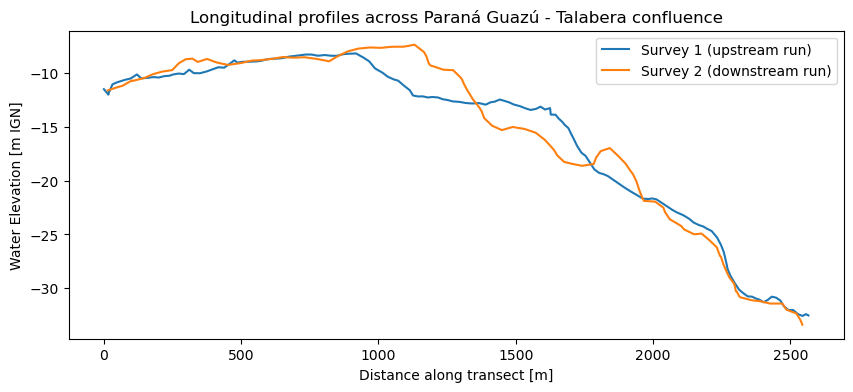
\includegraphics[width=0.75\linewidth]{figures/ch6/longitudinal profiles.png}
    \caption{Longitudinal profiles over dredging location at confluence of Paraná Guazú and Talabera}
    \label{fig:longitudinal profiles}
\end{figure}


\newpage
\section{Sediment Balance}
\label{sec: Sediment Balance}
In this section, the sediment balance of the region of interest will be derived. The control volume around the confluence of the Rió Paraná Guazú and the Río Talabera is shown in Figure \ref{fig:Area sediment balance}. The boundaries of this volume are defined by the cross sections in which discharge and sediment measurements were taken during fieldwork. These measurements are used to calculate the ingoing and outgoing sediment fluxes. As only measurements of a single day are available, the derived balance will be a momentary assessment of the amount of sediment entering and leaving the area, rather than a long-term sediment balance. However, since one of the main goals of this study is to investigate the effects of sand extraction on the river, a momentary sediment balance can still provide insights into the significance of the amount of sand that is being extracted.

\begin{figure}[H]
    \centering
    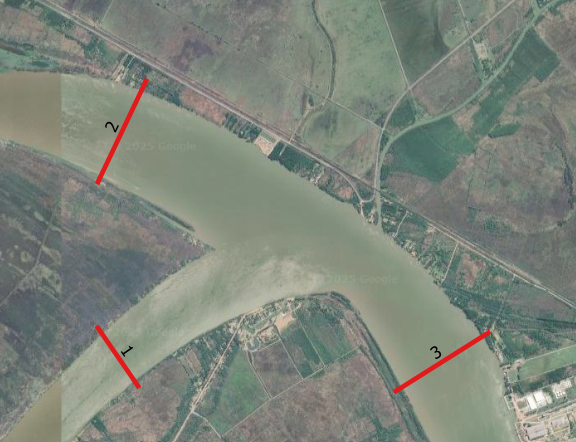
\includegraphics[width=0.75\linewidth]{figures/ch6/Map_sed_balance.png}
    \caption{Control volume for the sediment balance.}
    \label{fig:Area sediment balance}
\end{figure}

The computed suspended sediment fluxes from Section \ref{sec: Suspended sediment load} and bedload sediment fluxes from Section \ref{sec: Bed load} are shown in Table \ref{tab: Overview sediment fluxes}. From these fluxes, the total sediment flux per cross section is calculated, using Formula \ref{eq: Total sediment flux}. In addition, the total sediment flux in $kg/s$ is converted to a flux in tonnes per day, as the calculated flux is only representative of the day the measurements were taken. For all three cross sections it can be seen that suspended sediment largely contributes to the total sediment flux. For cross section 1 and 3 around 85\% of the total flux is suspended sediment. For cross section 2 this fraction is slightly lower with 74\%. 

\begin{equation}
    Q_t = Q_s + Q_b
    \label{eq: Total sediment flux}
\end{equation}

\begin{table}[H]
    \centering
    \caption{Overview of the computed sediment fluxes}
    \label{tab: Overview sediment fluxes}
    \setlength{\tabcolsep}{8pt}
    \begin{tabular}{c c c c c}
        \hline
        Cross Section & $Q_s~[kg/s]$ & $Q_b~[kg/s]$ & $Q_t~[kg/s]$ &  $Q_t~[tonnes/day]$ \\
        \hline
        1 & 121.38 &  18.43 & 139.81 & 12079.58\\
        2 & 76.17  &  26.92 & 103.09 & 8906.98\\
        3 & 342.76 & 60.32 & 403.08 & 34826.11\\
        \hline
    \end{tabular}
\end{table}

The volume of sand extraction estimated in Section \ref{sec: Dredging activities} is $100,000~m^3/month$. Using a sand density of $1600~kg/m^3$, the amount of sand extracted from the river yields $5333,33~tonnes/day$. Sand extraction in the river can be included in the sediment balance using the following formula:

\begin{equation}
    \Sigma Q_\text{t,in}  - \Sigma Q_\text{t,out} - Q_\text{Dredging}  = \Delta S \
    \label{eq: general formula sediment balance}
\end{equation}

In this formula, dredging is the only sink of sediment identified inside the control volume. There are no additional sources of sediment besides the computed fluxes. From Section \ref{sec: Longitudinal profiles} it was concluded that there is no sediment trapped in bars which can act as a sediment source. Local bank erosion is neglected as there is no information available and it is expected to be minimal on a daily scale.

By substituting the sediment fluxes from Table \ref{tab: Overview sediment fluxes} and the estimated sand extraction into Formula \ref{eq: general formula sediment balance}, the 
change in sediment storage ($\Delta S$) can be computed. The change in sediment storage is an indicator of net deposition (if positive) or net erosion (if negative).

\begin{subequations}\label{eq:sediment_balance}
    \begin{gather}
        Q_\text{t,1} + Q_\text{t,2} - Q_\text{t,3} - Q_\text{Dredging} = \Delta S \label{eq:sediment_balance_a} \\
        12079.58 + 8906.98 - 34826.11 - 5333.33 = \Delta S \label{eq:sediment_balance_b} \\
        -19{,}172.88~[\text{tonnes/day}] = \Delta S
        \label{eq:sediment_balance_c}
    \end{gather}
\end{subequations}

Due to the negative change in sediment storage, the deficit must be supplied by sediment already stored in the control volume, which causes bed/bank erosion. As the amount of sand extracted is $5333.33$ tonnes/day compared to the much larger $\Delta S$ of -$19,172.88$ tonnes/day, it can be concluded that the net erosion is not primarily caused by the sand extraction. Even without sand extraction, the system would still lack sufficient sediment to balance the deficit.

As the sediment balance is set up closely around the confluence, hydrodynamic effects at the confluence should be taken into consideration when interpreting the sediment balance. The meeting of two flows can create high turbulence and concentration of flow velocities. The increased turbulence enhances the sediment mixing and sediment resuspension, increasing the suspended sediment flux right after the confluence. Higher flow velocities as a result of a confluence, lead to an increased sediment carry capacity, which can potentially lead to scour of the river bed. The sediment deficit may be partly explained by the effects of the confluence still being present in the outgoing sediment flux.

As stated in Section \ref{sec: Suspended sediment load}, the calculations of the suspended sediment flux carry a lot of uncertainties. The computed sediment deficit is mostly caused by the ingoing and outgoing suspended sediment fluxes. If the ingoing fluxes are underestimated and the outgoing fluxes are overestimated, the resulting sediment balance will suggest an artificial sediment deficit. These uncertainties need to be taken into account when interpreting the sediment balance.


\section{Hydrodynamic effects on the River Banks}
\subsection{Aqua Monitor}
\label{section:cirtical_location}
In this section the data from the water gains and losses is explained in more detail.
Recalling the whole period of time available in Section \ref{Aqua Monitor Water Changes 1985-2025}, it is clear that the outer side of the river curves experience a water surface gain (indicated in blue), and the inner sides of the curves lose water, implying sedimentation (indicated in green). 
The location of the 'La Blanqueada' camping  is in the outer side of the curve near Puerto Constanza, as seen in the following Figure \ref{fig:Camping Blanqueada}.

\begin{figure}[H]
    \centering
    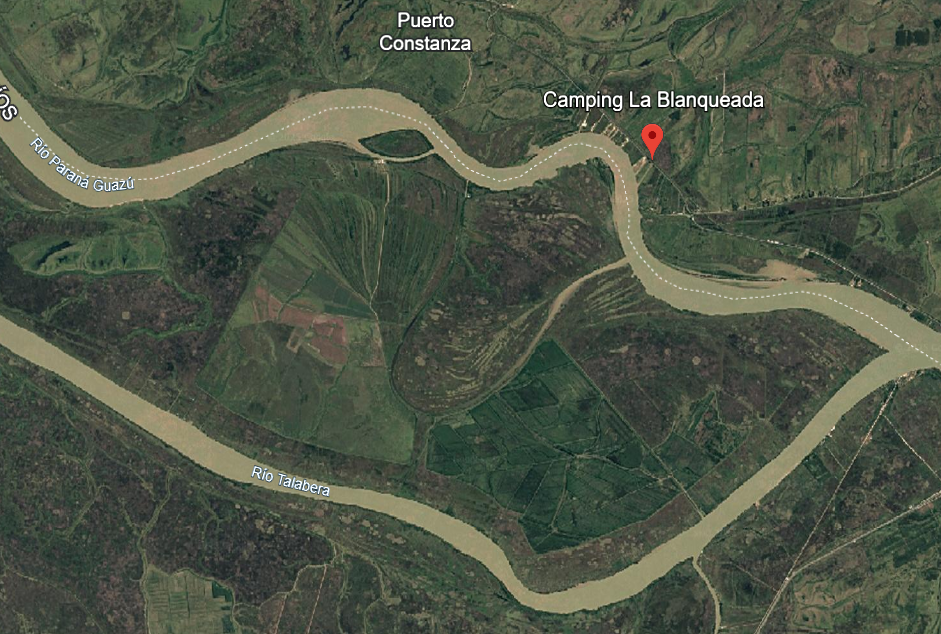
\includegraphics[width=0.5\linewidth]{figures/ch5/Camping Blanqueada.png}
    \caption{Location of the Camping La Blanqueada}
    \label{fig:Camping Blanqueada}
\end{figure}

The camping's location matches with the blue part of the water gain map, indicating that the water quantity around the shore of the camping has increased. 
In order to know if this has always been so, or if the water gains in this precise location have been gradually increasing, several maps with closer intervals have been created. 

There are quite a few comments to be made about the maps. First of all, blue and green zones stay consistent throughout the years, but when going into detailed time periods they can differ. Variations occur on shorter time periods such as the period 2005-2015, which indicated more water gains than losses in the deltas surrounding the region of interest. Another very interesting thing to note is that the flood of 2016 in the Parana Guazu can also be seen through the help of this map, on a time interval of 2015-2017.

Furthermore, droughts are also illustrated quite well with this application. The perfect example would be the long period of drought in 2022 which led some parts of the Parana to be left dry, as seen in Figure \ref{fig:Discharge Changes in Brazo Largo}. With the Parana Guazu's significant depths of over 40 meters this was unlikely to happen but still, this change in water quantity did not go unnoticed by the Deltares application. This can be seen on the Figure of 2020-2022.

Other periods of time are more or less stable and have nothing to report. For the sake of these explanations the relevant Figures can be found in the Appendix \ref{Appendix: Satellite Data}.

\begin{figure}[H]
    \centering
    \begin{subfigure}[a]{0.6\textwidth}
        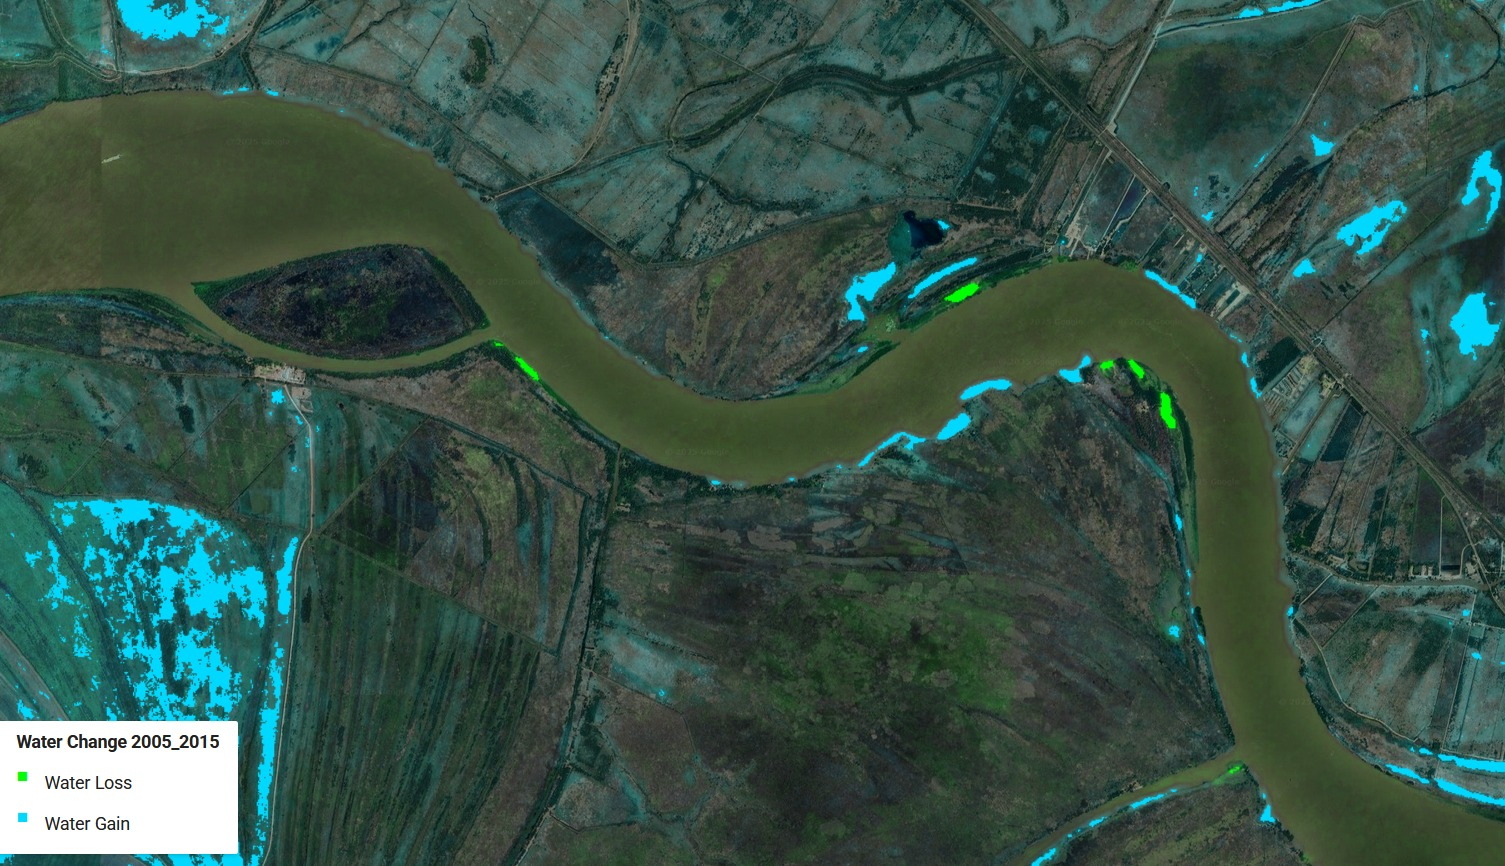
\includegraphics[width=\linewidth, height=5cm]{figures/ch5/2005-2015.jpg}
        \caption{Period 2005-2015}
        \label{fig:Period 2005-2015}
    \end{subfigure}
\end{figure}

\begin{figure}[H]
    \centering
    \begin{subfigure}[b]{0.6\textwidth}
        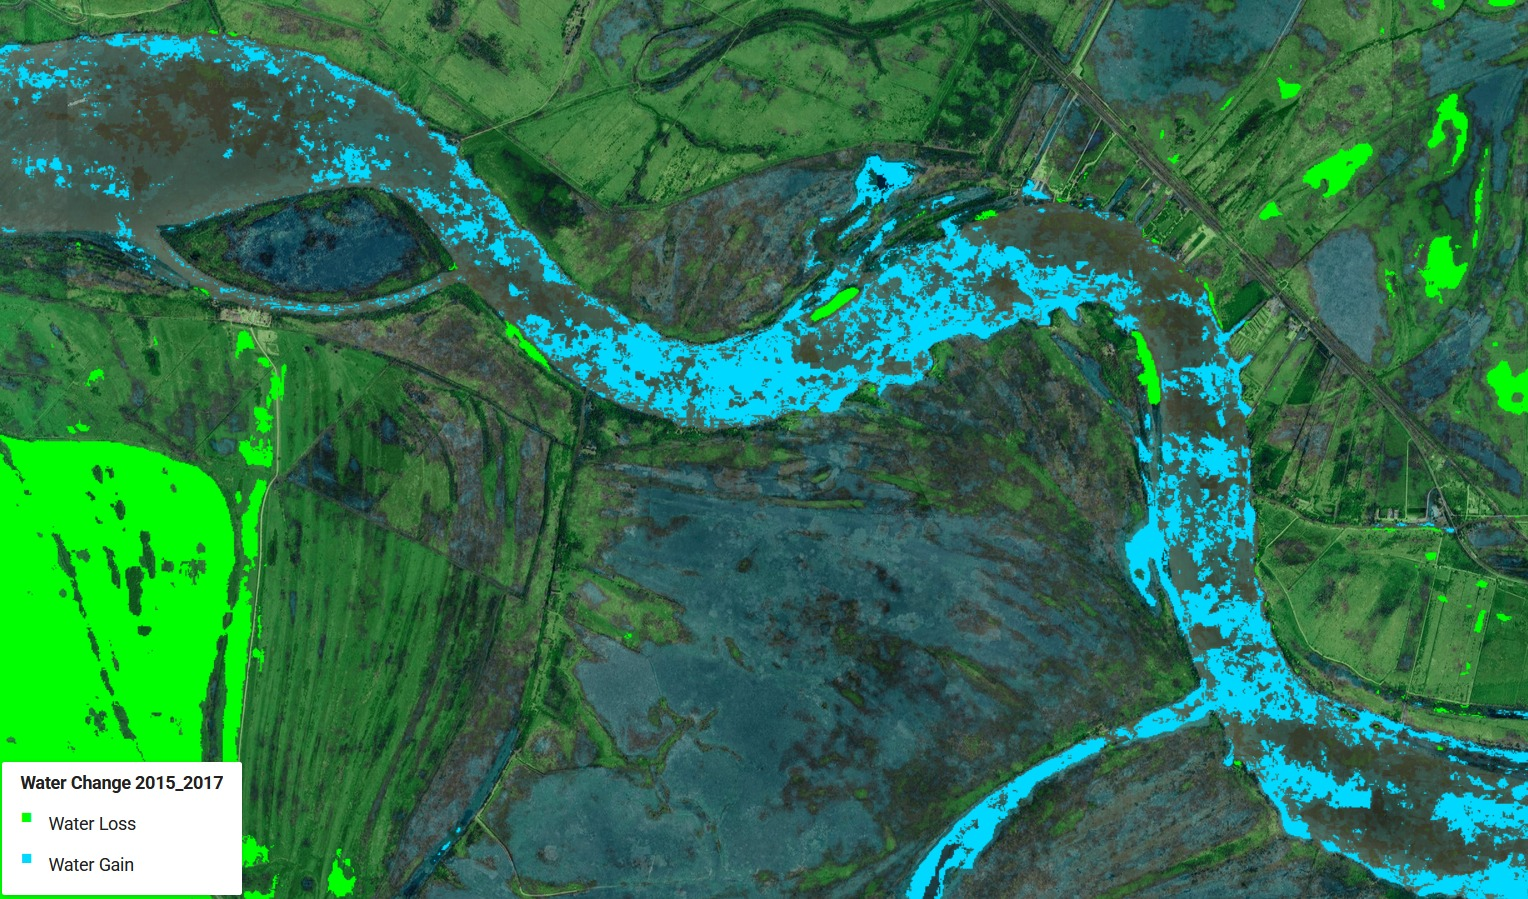
\includegraphics[width=\linewidth, height=5cm]{figures/ch5/2015-2017.jpg}
        \caption{Period 2015-2017}
        \label{fig:Period 2015-2017}
    \end{subfigure}
\end{figure}

\begin{figure}[H]
    \centering
    \begin{subfigure}[c]{0.6\textwidth}
        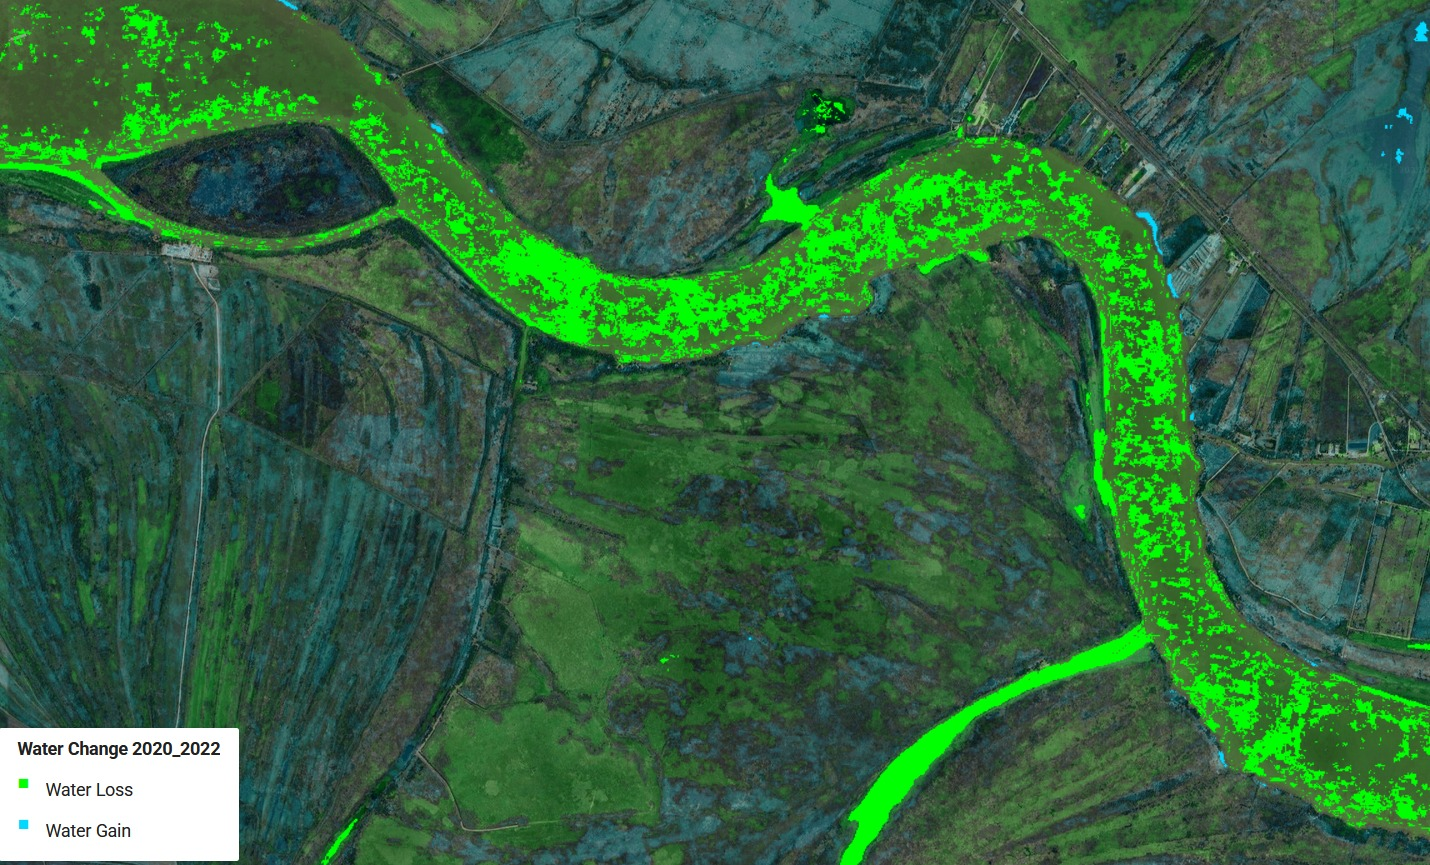
\includegraphics[width=\linewidth, height=5cm]{figures/ch5/2020-2022.jpg}
        \caption{Period 2020-2022}
        \label{fig:Period 2020-2022}
    \end{subfigure}
    
    \caption{Water Changes in Different Periods}
    \label{fig:Water Changes}
\end{figure}

\begin{figure}[H]
    \centering
    \begin{subfigure}{0.48\textwidth}
        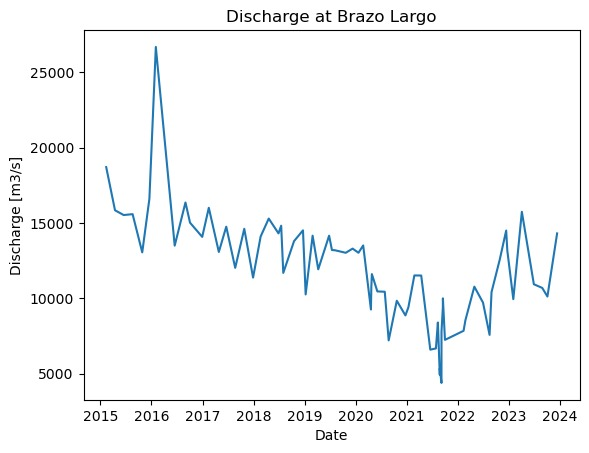
\includegraphics[width=\linewidth]{figures/ch5/dischargepeak.jpg}
    \end{subfigure}
    
    \caption{Discharge Changes in Brazo Largo}
    \label{fig:Discharge Changes in Brazo Largo}
\end{figure}




\subsection{Surface Area Measurements}
From the Aqua Monitor Software, one could establish which regions were of interest in a broad scope surrounding the Paraná Guazú bend near Puerto Constanza. Decreasing the scope leaves us with question marks regarding the actual areas and lengths of land that have been subject to these water gains. Therefore, it was chosen to investigate further into the details of the coast erosion with Google Earth.
Using the software's satellite data, one could draw a surface around the area of the Camping La Blanqueada in 2022, the most recent available, and then compare it to historical data. 
This gives a dataset of historical data from 1985 until 2022 but since the satellite images have been improving with time, the only relevant data can be taken from 2003 on.


Thus, it was chosen to take the difference in surface area from 2022 until 2003. Initially, only the East side of the camping was taken into account due to its matching with the drone pictures taken of the area during the field trip \ref{fig:Bank Erosion shots from field work}. Nevertheless on Google Earth it quickly became obvious that the necessity rose to take the West part of the Camping in consideration as well since its surface was eroded even further.

A summary of the data gathered from this study can be found in Figure \ref{fig:surface_comparison}. First the measurement of the East part of the Camping, then the comparison with 2003, 2017, 2018 and then for both sides the added surface lost since 2003.

\begin{figure}[H]
    \centering
    \begin{subfigure}[b]{0.45\textwidth} % Adjusted width to fit both images side by side
        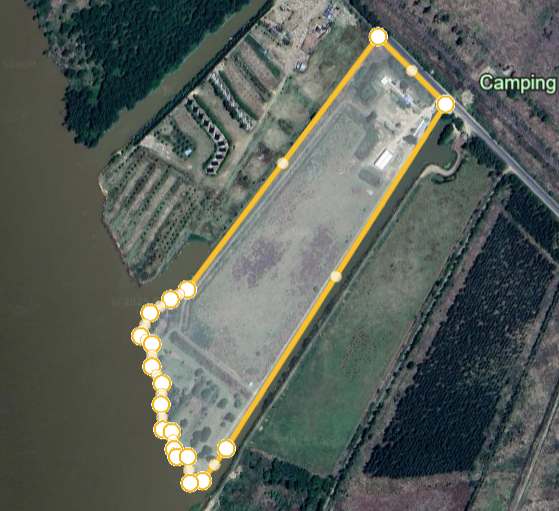
\includegraphics[width=\linewidth, height=5cm]{figures/appendix-g/opp2022.png}
        \caption{Surface Data for 2022}
        \label{fig:surface2022.2}
    \end{subfigure}
    \hfill
    \begin{subfigure}[b]{0.45\textwidth} % Adjusted width to fit both images side by side
        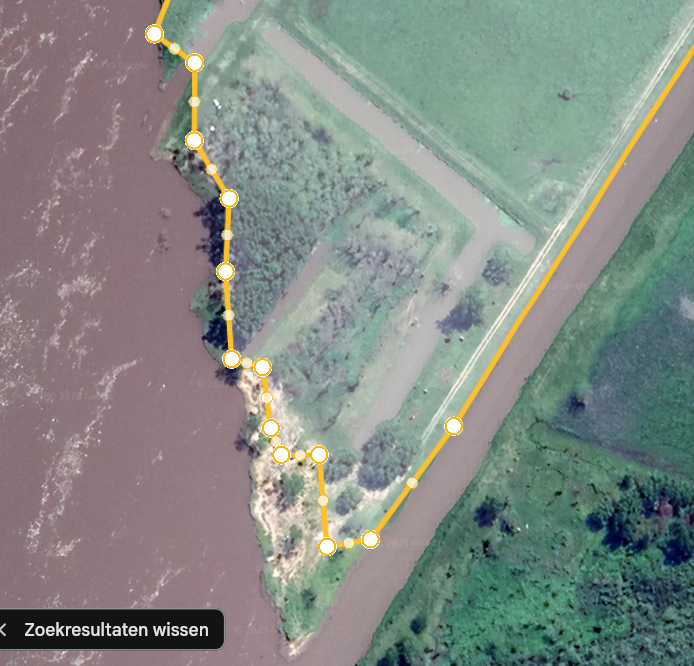
\includegraphics[width=\linewidth, height=5cm]{figures/appendix-g/opp2017.png}
        \caption{Surface Data for 2017}
        \label{fig:surface2017}
    \end{subfigure}
    \hfill
    \begin{subfigure}[b]{0.45\textwidth} % Adjusted width to fit both images side by side
        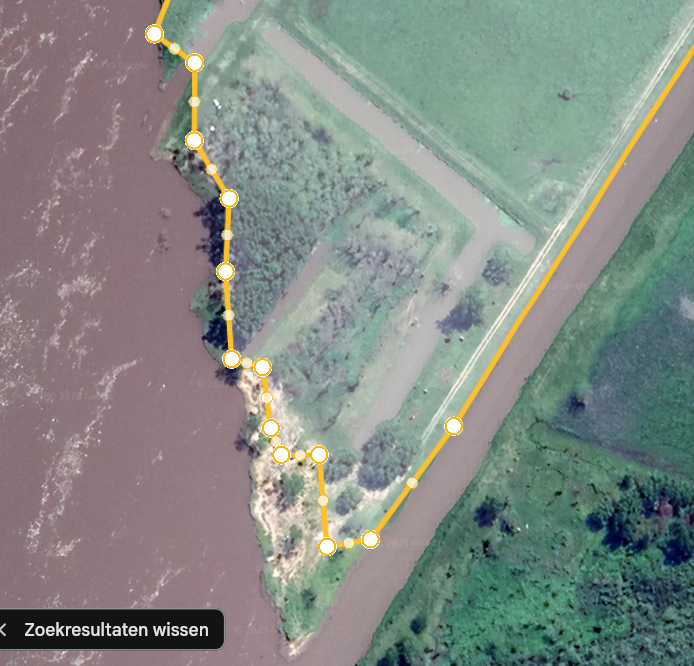
\includegraphics[width=\linewidth, height=5cm]{figures/appendix-g/opp2018.png}
        \caption{Surface Data for 2018}
        \label{fig:surface2018}
    \end{subfigure}
    \hfill
    \begin{subfigure}[b]{0.45\textwidth} % Adjusted width to fit both images side by side
        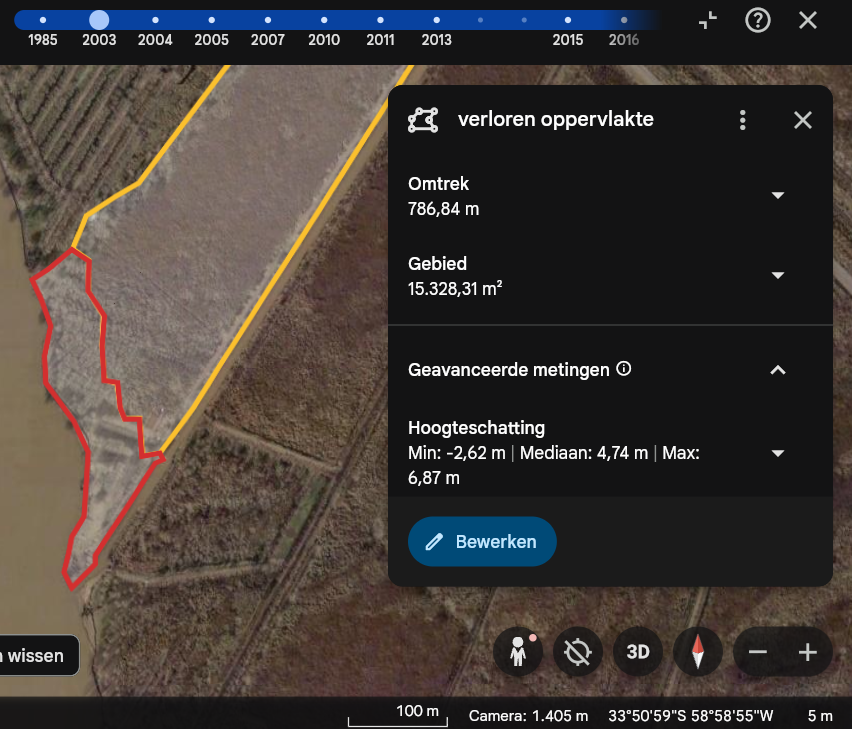
\includegraphics[width=\linewidth, height=5cm]{figures/appendix-g/verlorenopp2003.png}
        \caption{Surface Data for 2003}
        \label{fig:surface2003.2}
    \end{subfigure}
    \caption{Comparison of Surface Data}
    \label{fig:surface_comparison}
\end{figure}

It is known that there was a flood in 2016 \autocite{equipodemanejodeinformacionArgentinaInundaciones2016}. This flood was in return responsible for a significant increase of water quantity and discharge throughout the region, as seen in Figure \ref{fig:Discharge Changes in Brazo Largo}. Consequently, this affected certain areas of the channel more than others, in particular the curves of the Parana Guazu such as Puerto Guazu showed in the Figures \ref{fig:Water Changes}. The negative impacts were highlighted when the high discharge and water quantities dropped back to normal, leaving a part of the bank fragile which then contributed to an accelerated bank erosion. This argument can once again be solidified by the drastic increase of erosion in between those time periods. After this flood event, the rate of erosion decreased again.

Lastly, both sides of the Camping and the difference between 2003 and 2022 can be seen below. The leftover piece of land which was present in 2003 but has been eroded since then is also traced as a surface area in a distinct colour (see Figure \ref{fig:surfacelost_comparison}). The complete comparison with all accessible historical data was documented in the Appendix \ref{Appendix: Satellite Data}. Moreover, values of the surface areas, perimeters, and further quantification's can be found in Section \ref{section:quantitative_results}.

\begin{figure}[H]
    \centering
    \begin{subfigure}[b]{0.45\textwidth} % Adjusted width to fit both images side by side
        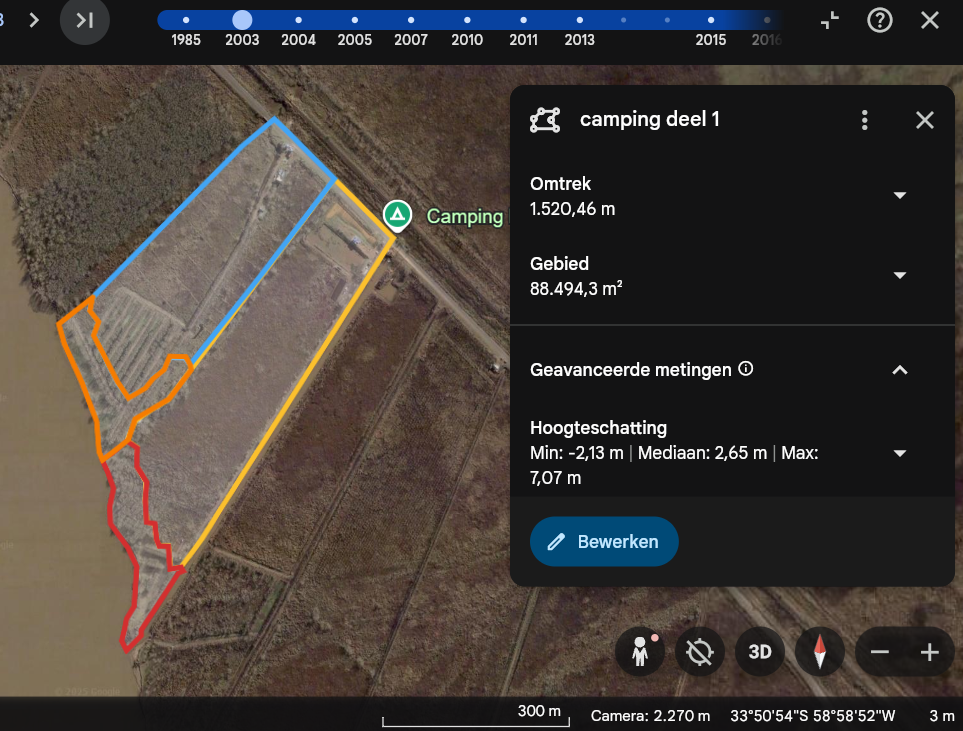
\includegraphics[width=\linewidth, height=5cm]{figures/appendix-g/delen2003.png}
        \caption{Surface Data for 2003}
        \label{fig:surface2003.1}
    \end{subfigure}
    \hfill
    \begin{subfigure}[b]{0.45\textwidth} % Adjusted width to fit both images side by side
        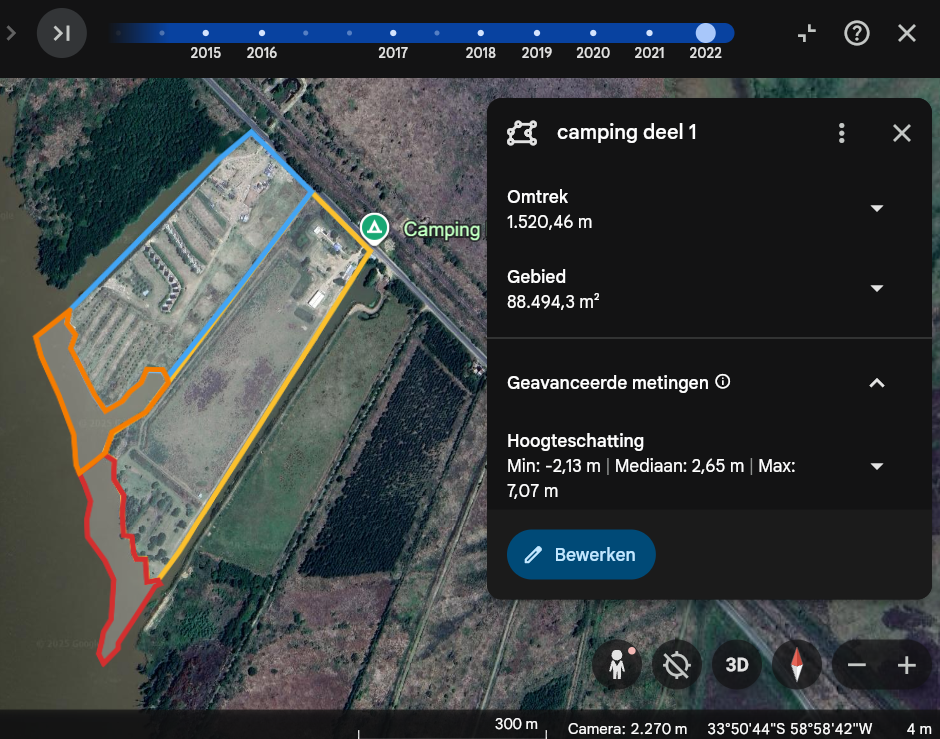
\includegraphics[width=\linewidth, height=5cm]{figures/appendix-g/delen2022.png}
        \caption{Surface Data for 2022}
        \label{fig:surface2022.1}
    \end{subfigure}
    \caption{Comparison of Lost Surface Data}
    \label{fig:surfacelost_comparison}
\end{figure}


\subsection{Quantitative Results}
\label{section:quantitative_results}

The values of these areas can be found in the Table \ref{tab:Surface Lost Camping La Blanqueada in 2022}.
Do keep in mind that the green part of the area is very likely to be digged out by the owner himself to build a channel for the boats. This probably contributes to an acceleration of the erosion around it, but it is still relevant to mention.

\begin{table}[H]
\centering
\caption{Surface Recap Camping La Blanqueada in 2022}
\label{tab:Surface Lost Camping La Blanqueada in 2022}
\begin{tabular}{l l l S[table-format=5.2] S[table-format=5.2]}
\toprule
Location & Category & Colour & Perimeter (m) & Area (m²) \\
\midrule
East Part & Actual & Yellow & 1520.46 & 88494.3 \\
East Part & Lost & Red & 786.84 & 15328.31 \\
West Part & Actual & Blue & 1203.31 & 71231.39 \\
West Part & Lost & Orange & 466.7 & 8698.71 \\
West Part & Dug out & Green & 468.46 & 7622.01\\
\bottomrule
\label{Table: Surface Recap Camping La Blanqueada in 2022}
\end{tabular}
\end{table}

In addition to that, the lengths of the lost land can be found using the ruler in Google Earth as well. This gives the possibility of illustrating the scale of the erosion, and how much the owners of the Camping lost their land in the last decades. 
In the most extreme case down south east of the camping zone, which can be seen in the Figure \ref{fig:surfacelost_comparison} by the purple lines, and once again in more detail in Figure \ref{fig:lengthlost_comparison}.


\begin{figure}[H]
    \centering
    \begin{subfigure}[b]{0.45\textwidth} % Adjusted width to fit both images side by side
        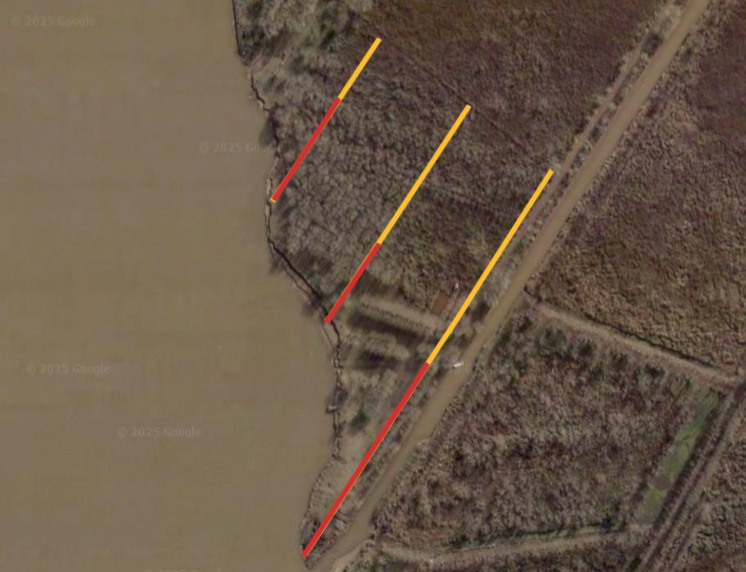
\includegraphics[width=\linewidth, height=5cm]{figures/ch5/length2003.png}
        \caption{Length of Land 2003}
        \label{fig:length2003}
    \end{subfigure}
    \hfill
    \begin{subfigure}[b]{0.45\textwidth} % Adjusted width to fit both images side by side
        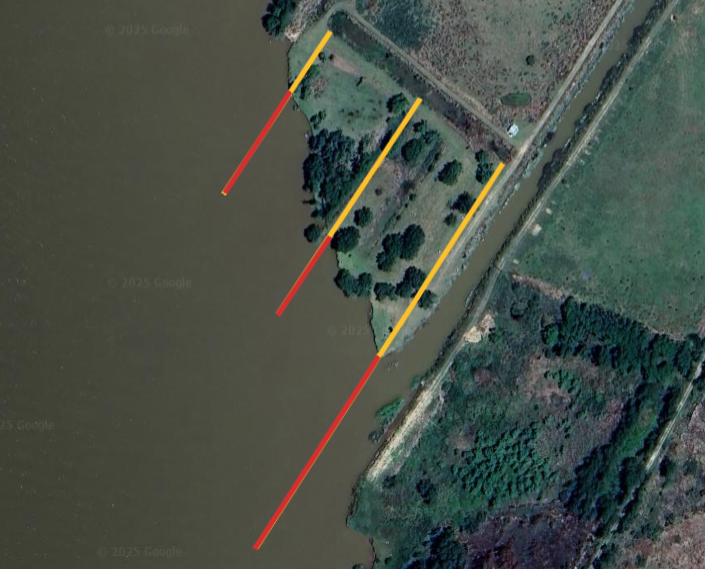
\includegraphics[width=\linewidth, height=5cm]{figures/ch5/length2022.png}
        \caption{Length of Land 2022}
        \label{fig:length2022}
    \end{subfigure}
    \caption{Comparison of Lost Surface Data}
    \label{fig:lengthlost_comparison}
\end{figure}

The lengths of the measured segments as well as the lost length have been calculated and put in the Table \ref{Table:Loss of Land for Camping La Blanqueada in 2022} below.


\begin{table}[H]
\centering
\caption{Loss of Land for Camping La Blanqueada in 2022}
\begin{tabular}{l l c}
\toprule
Location & Length in 2003 (m) & Loss of Length in 2022 (m) \\
\midrule
Section 1 & 118  & 73 \\
Section 2 & 156 & 57 \\
Section 3 & 276 & 138 \\
\bottomrule
\label{Table:Loss of Land for Camping La Blanqueada in 2022}
\end{tabular}
\end{table}

Lastly, the loss ratio's of the Camping surface are calculated in the Appendix \ref{Appendix: Satellite Data}. 

\subsection{Qualitative Results}
From this data, one can see that for the camping there has been a loss of 57 to 138 meters on the bank of the land. Some parts are more extreme than others, but on the whole from 2003 to 2022 this amount of land loss is worrying.

First of all, it is important to ask how this happened and what factor or problem contributes the most to the calculated erosion. The group started from a quite biased point of view only taking into account the opinion of the stakeholders. They gave away that the reason for this erosion was purely the dredging of the sand and the cargo ships passing by. From the Wave impact study it shows that the cargo ships induced waves do in fact contribute to the bank erosion when passing by. It is quite hard to determine how much faster the erosion is happening due to this event but one might assume the fact that the contribution to the problem is small, but not insignificant. Moreover, it is important to take into account the fact that the likelihood of the digging for a boat channel for the camping adds onto the erosion of the shore.

The Aqua Monitor study illustrates the high correlation between the water levels and discharge intensities with the water quantities gained in certain areas. The borders of curves in a channel are the most likely to be victim of the water gains which makes the bank stability decrease when the hydro parameters discharge and water quantity are restored to a normal level, as explained in the section \ref{chap 6: effect on the river bed}. From this part, one can assume that after a flood, the banks become even more fragile and break apart at a faster pace after the flood is gone.
In addition to that, one can also state that this major factor contributing to bank erosion as the satellite data shows in Figure \ref{fig:surface_comparison}.

It is also relevant to note that the number of flooding occurrences is positively correlated with climate change. This is because warmer temperatures cause more water to evaporate from the land and oceans, as well as changes in the size and frequency of heavy precipitation events. Thus, more extreme droughts, evaporation, and precipitations lead to more extreme floods \autocite{usenvironmentalprotectionagencyClimateChangeIndicators2016}.

Lastly, the natural erosion of a river has to be taken seriously when analysing this problem. Since the study area part of the river has meanders, it is normal to have some erosion on the outsides of the curves and deposition on the inside of the turns, due to the water with sediment passing by. The reason behind it is that water flows fast on the outside, leading to more erosion. On the inside, the water flows slowly, and thus making it easier for sediment to be deposited. Overtime, this creates more wider turns, explaining the erosion on the outside curve near the Camping of La Blanqueada \autocite{serenani}.

Therefore, climate change and natural erosion are the significant factors that contribute to bank erosion, and not the passing of cargo ships, nor the dredging of the sand a few hundred meters from the Camping La Blanqueada.
The situation was analysed for this very precise location. Other parameters may be taken into account when establishing this reasoning on another section of the Parana Guazu, but the method can be the same and the satellite images as well as the Aqua Monitor are accessible for every location. 

 